%% International Journal of Computational Intelligence Systems ---
%%%%%%%%%%%%%%%%%%%%%%%%%%%%%%%%%%%%%%%%%%%%%%%%%%%%%%%%%%%%%%%%%%%%%%%%%%%
\documentclass[11pt,twoside]{article}
\usepackage{ijcis}
%--------------------- ADDITIONAL PACKAGES HERE ---------------------------
\usepackage{amsmath}
\usepackage{amssymb}
\usepackage{color}

\hyphenation{pro-per-ties}
\hyphenation{ge-ne-ral-ly}
\hyphenation{pre-fe-ren-ces}
\hyphenation{u-sing}
\hyphenation{pu-nish-ment}
\hyphenation{vo-ca-bu-la-ry}
\newcommand{\Pow}{\mathcal{P}}
\newcommand{\N}{\operatorname{N}}
\newcommand{\bool}{\operatorname*{\mathcal{B}}}
\newcommand{\Pos}{\operatorname{Pos}}
\newcommand{\Nec}{\operatorname{Nec}}
\newcommand{\Open}{\operatorname{Open}}
\newcommand{\Rp}{\operatorname{Rp}}
\newcommand{\Rn}{\operatorname{Rn}}
\newcommand{\FB}{\operatorname{FB}}
\newcommand{\UC}{\operatorname{UC}}
\newcommand{\T}{\mathcal{T}}
\newcommand{\Rel}{\mathcal{R}}
\newcommand{\C}{\mathcal{C}}
\newcommand{\Nat}{\mathbb{N}}
\newcommand{\Q}{\mathbb{Q}}
\newcommand{\R}{\mathbb{R}}
\newcommand{\Z}{\mathbb{Z}}
\newcommand{\Head}{\mathcal{H}}
\newcommand{\Body}{\mathcal{B}}
\newcommand{\Dom}{\mathcal{D}}
\newcommand{\INS}{\mbox{\textbf{insert}}}
\newcommand{\DEL}{\mbox{\textbf{delete}}}
\newcommand{\MOD}{\mbox{\textbf{modify}}}
\newcommand{\REV}{\mbox{\textbf{revise}}}
\newcommand{\Overlap}{\mbox{\textbf{Overlap}}}
\newcommand{\A}{\mathcal{A}}
\newcommand{\I}{\mathcal{I}}
%--------------------------------------------------------------------------
%
\def\labart{yourLabel}      % put a label from your choice here
%\Vol{1}                    % number of the Volume
%\Issue{1}                  % number of the issue
%\Month{January}            % month
%\Year{2008}                % year
%\received{...}
%\revised{...}
%
%---------------------------------------------------------------------------
\thispagestyle{empty}
%%------------------------- YOUR HEADINGS HERE -----------------------------
% Author's initials of first names+last names
\shortauthors{J. Pons, C. Billiet, N. Mar\'{i}n,  O. Pons,  G. De Tr\'{e}}
% Short title
\shorttitle{A Relational Model for the Possibilistic Valid-time Approach}
%---------------------------------------------------------------------------
%
%---------------------- YOUR TITLE ----------------------------------------
\title{A Relational Model for the Possibilistic Valid-time Approach} 
% \\ \vspace*{0.04truein}
%Using \LaTeX\footnote{For the title, try not to use more than 3 lines.
%Typeset the title in 12 pt Times Roman, uppercase and boldface.}
%
%-------------------------- AUTHOR'S NAMES ----------------------------------
\author{%
Jose Enrique Pons*\,\up{1}, Christophe Billiet\,\up{2}, Nicol\'{a}s Mar\'{i}n\,\up{1},  Olga Pons\,\up{1}, Guy de Tr\'{e}\,\up{2}
}
%----------------------------- ADDRESSES ----------------------------------
\addresses{%
%\address{
\up{1}
Department of Computer Science and Artificial Intelligence, University of Granada\\
C/ Periodista Daniel Saucedo Aranda, S/N,E-18071\\
Granada, Spain%
\footnote{
Corresponding author.
%State completely without abbreviations, the affiliation
%and mailing address, including country. Typeset in 10~pt Times Italic.
}
\\ \vspace*{0.04truein}
E-mail: jpons,opc,nicm@decsai.ugr.es\\
%}\address{%
%\\ \vspace*{0.05truein}
\up{2}
Department of Telecommunications and Information Processing, Ghent University \\
Sint-Pietersnieuwstraat 41, \\ B-9000, Ghent, Belgium.
%\\ \vspace*{0.04truein}
\\ E-mail: Christophe.Billiet, Guy.De.Tre@ugent.be
}
%---------------------------------------------------------------------------
\pagestyle{myheadings}
\begin{document}
\label{\labart-FirstPage}

\maketitle
%-------------------------- ABSTRACT ---------------------------------------
\abstracts{
%%%%%%%%%%%%%%%%%%%%%%%%
%
% ABSTRACT
%
%%%%%%%%%%%%%%%%%%%%%%%%
In real world, it is very common that some objects or concepts have properties with a time-variant or time-related nature. Modelling this kind of objects or concepts in a (relational) database schema is possible, but time-variant and time-related attributes have an impact on the consistency of the entire database and have to be appropriately managed. Therefore, temporal database models have been proposed to deal with this problem in the literature. Time can be affected by imprecision, vagueness and / or  uncertainty, since existing time measuring devices are inherently imperfect. Additionally, human beings manage time using temporal indications and temporal notions, which may also be imprecise. However, the imperfection in human-used temporal indications is supported by human interpretation, whereas information systems need appropriate support in order to accomplish this task. Several proposals for dealing with such imperfections when modelling temporal data exist. Some of these proposals transform the temporal data into a compact representation but there is not a formal model for managing and handling uncertainty regarding temporal information.
In this work we present a novel model to deal with imprecision in valid-time databases together with the definition and implementation of the data manipulation language, \emph{DML}.
%
%The abstract should summarize the context, content and conclusions of the
%paper in less than 80 words. It should not contain any references or
%displayed equations. Typeset the abstract in 9~pt Times Roman with
%baselineskip of 11 pt, making an indentation of 2.5 picas on the left
%and right margins.
}
\par\bigskip\par
%-------------------------- KEYWORDS ---------------------------------------
\keywords{fuzzy, temporal, database}

\vspace*{10pt}\textlineskip
%-------------------------- BEGIN BODY OF TEXT -----------------------------
\begin{multicols}{2}

\section{\label{sec:intro}Introduction}
%%%%%%%%%%%%%%%%%%%%%%%%%%%%%%%%%%%%%%%%%%%%%%%%%%%%%%%%%%%%%%%%%%%%%%
%
% Introduction
%
%%%%%%%%%%%%%%%%%%%%%%%%%%%%%%%%%%%%%%%%%%%%%%%%%%%%%%%%%%%%%%%%%%%%%%
The concept of \emph{time} is easy to understand but very complex to define~\cite{klein94}~\cite{Shackle61}. 
In Information Systems \emph{IS}, several proposals have been concerned with the obtaining of theoretical models that allow the representation of time~\cite{Bolour82}~\cite{Cru97}. 
More towards temporal databases, a lot of work have been done. The first efforts were towards the representation of the historical information related to an object in the database(reference). Some works tried to extend the Entity Relationship Model \emph{ERM} ~\cite{Klopprogge:1983} but without an impact on any database standards like SQL~\cite{Sarda:1990:ESH:627277.627409}.

The ``Consensus Glossary of Temporal Database concepts'' \cite{Dyreson1994} is the first publication where the main researchers in temporal databases define the main thesaurus of temporal database concepts. This glossary defines the main types of time in a temporal database and is the basis of furthers researches ~\cite{Sarda:1990:ESH:627277.627409} \cite{Jensen94thetsql2}.

Another main issue in temporal databases is the querying. The user specifies in the query some temporal constraints, e.g. \emph{``before this year''},\emph{``after 1995''}. In order to solve these temporal comparisons, between the time specified in the query and the temporal data stored in the database, some basic relationships have been defined. Allen~\cite{Allen83} first introduced the temporal relations between time intervals and, to a lesser extent, to time points. Some authors~\cite{ohlbach2004},\cite{nagypal2003},\cite{schockaert08} have softened the temporal operators defined by Allen. Therefore it is possible to compute the relationships between two ill-known time points or intervals. In~\cite{garrido2009}, some different temporal operators are defined by a combination of regular fuzzy comparisons. %e.g. the \emph{BEFORE} operator is defined by means of the fuzzy less than (FLT) operator. 

To allow information systems to cope with uncertainty, many approaches adopt fuzzy sets~\cite{Zadeh65} for the representation of temporal information~\cite{Billiet:Pons:Matthe:DeTre:Pons:2011:BipolarFuzzy},\cite{Dubois:jucs_9_9:fuzziness_and_uncertainty_in},~\cite{devos94}. The time points representing the time when the object is valid in the reality might not be precisely known. In order to deal with this, several models have been proposed. Garrido~\cite{garrido2009} proposes a model to deal with uncertainty in the time interval by means of fuzzy intervals. Bronselaer~\cite{Pon11} proposes a consistent framework to deal and represent ill-known time values and their relationships. Rough sets~\cite{Pawlak1995} have been also used to represent time intervals~\cite{Qia09} in databases.

%temporal reasoning and fuzzy temporal reasoning.
Next to the manage of temporal information is the temporal reasoning~\cite{Allen83}. Dubois and Prade ~\cite{Dubois:jucs_9_9:fuzziness_and_uncertainty_in},\cite{Dubois89} deal with fuzzyness and uncertainty in temporal reasoning, but this topic is outside the scope of this work.

%temporal commercial systems.

The work is organized as follows: 

In Section \ref{sec:time-domain} an study about the time and its properties is done. Section \ref{sec:temporal-databases} is an overview of the main problems when managing the time in a database, the different proposals for solving them and the temporal database proposals. The section concludes with a comparison among the different proposals. In Section \ref{sec:fuzzy-temporal-databases} we present a sum up with the proposals for handling the imprecision in temporal databases and the main deficiences we have detected. Finally, there are several commercial temporal database management systems  \emph{TDMBS} like \cite{oracle2009},\cite{posgree2009},\cite{teradata2011},\cite{timedb2005}. All of them are analyzed and compared later on this work. 



\section{\label{sec:prelim}Preliminaries}
%Introductory text:
In this section, we introduce some basic concepts concerning possibilistic variables and fuzzy numbers and intervals. Then, the framework of set evaluation by ill-known constraints \cite{Pons2011} is explained. The section concludes with a brief introduction to temporal databases.


% %Something about relational databases in general and relations in specific (to make the vocabulary clear)
% \subsection{Relational Databases}
% In this subsection, a few structural and behavioral aspects of the relational database model will be presented.
% 
% In a relational database, information is structured in \emph{relations}. As explained in the introduction, a collection of similar entities is modelled by an entitytype, which, using the relational database model, will be modelled by a relation. A relation consists of a \emph{relation schema} and an \emph{extention}. The relation schema basically determines the relation structure, by dictating which data (describing entities) will be kept and how these data will be represented. Each (atomic) part of these data is a result value of a measurement of a property of an entity or a description of a property of an entity. The extention contains these data. A relation schema consists of a \emph{relation name} and a finite set of \emph{attributes}. The relation name is of course the name of the entire relation, while the attributes describe common properties of the entities modelled by the relation. Every attribute consists of an attribute name and an associated \emph{data type}. Each data type has its \emph{domain} and its operators. The domain of a data type is the set of values which data of the data type in question can assume. Operators of a data type can be applied to data of a data type. The extention of a relation is a set of \emph{tuples}. Each tuple represents an enitity, by containing values: for every attribute in the attribute set of the relation schema, the tuple contains the value describing the exact state of the property of the entity. %Remember: a tuple is just an ordered tuple of values.

\subsection{\label{subsec:possibility-theory}Possibility Theory}
Possibility theory is devoted to the handling of incomplete information. In order to capture partial ignorance, two measures are provided: possibility and necessity.

\begin{definition}
Consider a set of outcomes $\Omega$. Let $\wp(\Omega)$ denote the powerset of $\Omega$ and let $A$ and $B$ be elements of $\wp(\Omega)$. A \emph{confidence measure on $\Omega$} is defined by a function
	\begin{align}
	g : \wp(\Omega) & \rightarrow \left[0,1\right]
	\end{align}
that satisfies
	\begin{align}
	g(\emptyset) &= 0 \\
	g(\Omega) &= 1 	\label{NormalizationProperty} \\
	A \subseteq B &\Rightarrow g(A) \leq g(B) \label{MonotonicityProperty}
	\end{align}
\end{definition}

Both possibility and necessity measures are special cases of confidence measures.



\begin{definition}
Consider a confidence measure $\Pi$ on a set of outcomes $\Omega$. Let $J$ be a countable index set and let $\{ A_{j} | j \in J \wedge A_{j} \subseteq \Omega \}$ be a family of elements of $\wp(\Omega)$. $\Pi$ is now a \emph{possibility measure on $\Omega$} if it satisfies:
	\begin{align}
	\Pi\left(\bigcup_{j \in J} A_{j} \right) = \sup_{j \in J} \Pi(A_{j})
	\end{align}
\end{definition}

In this work, the interpretation is as follows. The possibility of an event expresses how plausible the occurrence of the event seems to an observer of the experiment, given the (partial) knowledge of the observer about the experiment.

Information on the possibility of distinct elements of the universe of discourse $\Omega$ can now be given by a \emph{possibility distribution} $\pi$ on $\Omega$, defined by:

\begin{definition}
Consider a possibility measure $\Pi$ on $\Omega$. A \emph{possibility distribution} $\pi$ on $\Omega$ underlying the possibility measure $\Pi$ is a function defined by:
	\begin{align}
	\pi : \Omega \rightarrow \left[0, 1\right] : \pi(u) = \Pi(\{u\})
	\end{align}
\end{definition}

\begin{definition}
Consider a confidence measure $N$ on $\Omega$. Let $J$ be a countable index set and let $\{ A_{j} | j \in J \wedge A_{j} \subseteq \Omega \}$ be a family of elements of $\wp(\Omega)$. $N$ is a \emph{necessity measure} on $\Omega$ if it satisfies:
	\begin{align}
	N\left(\bigcap_{j \in J} A_{j} \right) = \inf_{j \in J} N(A_{j})
	\end{align}
\end{definition}

In this work, the interpretation is as follows. The necessity of an event expresses how necessary the occurrence of the event seems to an observer of the experiment, given the (partial) knowledge of the observer about the experiment.

Possibility and necessity measures are dual in the sense that:

\begin{align}
\forall A \subseteq \Omega : N(A) = 1 - \Pi(\bar{A})
\end{align}

That is, the degree to which an event is necessary is the extent to every other possible event is not plausible.

\subsection{\label{subsec:possibilistic-variables}Possibilistic Variables}
Possibilistic variables rely on possibility theory \cite{Dubois1988a} and are defined as follows \cite{Pons2011}.

\begin{definition}
\label{def;possibilistic-variable}
A possibilistic variable $X$ over a universe $U$ is defined as a variable taking exactly one value in $U$, but for which this value is (partially) unknown. Possibility distribution $\pi_X$ on $U$ models the available knowledge about the value $X$ takes; for each $u\in U$, $\pi_X(u)$ represents the possibility that $X$ takes the value $u$. In this work, this possibility is interpreted as a measure of how plausible it is that $X$ takes the value $u$, given (partial) knowledge about the value $X$ takes.
\end{definition}

The exact value a possibilistic variable takes, which is (partially) unknown, is called an \emph{ill-known value} in this work \cite{Dubois1988a}.

When a possibilistic variable is defined on the powerset $\Pow(U)$ of some universe $U$, the unique value the variable takes will be a crisp set and its possibility distribution on the powerset $\Pow(U)$ will describe the possibility of each crisp subset of $U$ to be the value the variable takes. This exact value (a crisp set) the variable takes, is now called an \emph{ill-known set} \cite{Dubois1988a}.

% It is important to understand the difference between the following two concepts:
% \begin{itemize}
% \item
% A \emph{possibilistic variable} $X$ is bounded to take only one value , but this value is not known due to incomplete knowledge. 
% \item
% An \emph{ill-known set}~\cite{Dubois1988a}: a possibilistic variable defined over the universe $\Pow(U)$.
% \end{itemize}

Note that while a possibilistic variable refers to one (partially) unknown value, an ill-known set is a crisp set but, for some reason, (partially) unknown.

A specific application of possibilistic variables is obtained when the universe under consideration is the set of Boolean values $\mathbb{B}$ = $\{T,F\}$. Indeed, any Boolean proposition $p$ takes just one value in $\mathbb{B}$. If the knowledge about which value this proposition $p$ will take is given by a possibility distribution $\pi_p$; the proposition can be seen as a possibilistic variable. The possibility and necessity that $p$ = $T$ (the proposition holds) demand more attention. This possibility and necessity is noted here as:
\begin{align}
\label{propholdsposs}
\text{Possibility that $p$ = $T$ (p holds):} &\\
\nonumber
Pos(p) = \pi_p(T)  \\
\label{propholdsnecc}
\text{Necessity that $p$ = $T$ (p holds):} & \\
\nonumber
Nec(p) = 1-\pi_p(F) 
\end{align}

Here, equation \eqref{propholdsposs} denotes the possibility that $p$ = $T$ and the proposition holds, while equation \eqref{propholdsnecc} denotes the necessity that $p$ = $T$ and the proposition holds.

This work deals with ill-known intervals. These are ill-known sets, defined and represented via a starting and ending points that, in turn are ill-known values. The elements of the set are the values between the starting and ending points. A closed ill-known interval with starting point defined by possibilistic variable $X$ and ending point by possibilistic variable $Y$ is noted here $\left[X, Y\right]$. %The correspondences and transitions between the representations of ill-known sets, between the representations of ill-known intervals and between the representations of an ill-known set and an ill-known interval are part of the authors current research.

\subsection{\label{subsec:fuzzy-numbers}Fuzzy Numbers and Fuzzy Intervals}
Among others, Dubois and Prade~\cite{Dubois1983} use fuzzy sets \cite{Zadeh1965} to define a \emph{fuzzy interval}:
\begin{definition}
A fuzzy interval is a fuzzy set $M$, defined by a membership function $\mu_{M}$ on the set of real numbers $\mathbb{R}$ such that:
\begin{eqnarray}
\mu_{M} :  \mathbb{R} \rightarrow \left[0,1\right]  \\ 
\nonumber
\forall (u,v)\in\mathbb{R}^2: \forall w \in [u,v]:\\
\nonumber
\mu_M(w) \geq\min(\mu_M(u),\mu_M(v))  \\
\nonumber
\exists m \in \mathbb{R} :  \mu_M(m)=1 
\end{eqnarray}
\end{definition}

\begin{samepage}
\vspace*{13pt}
\begin{center}
{
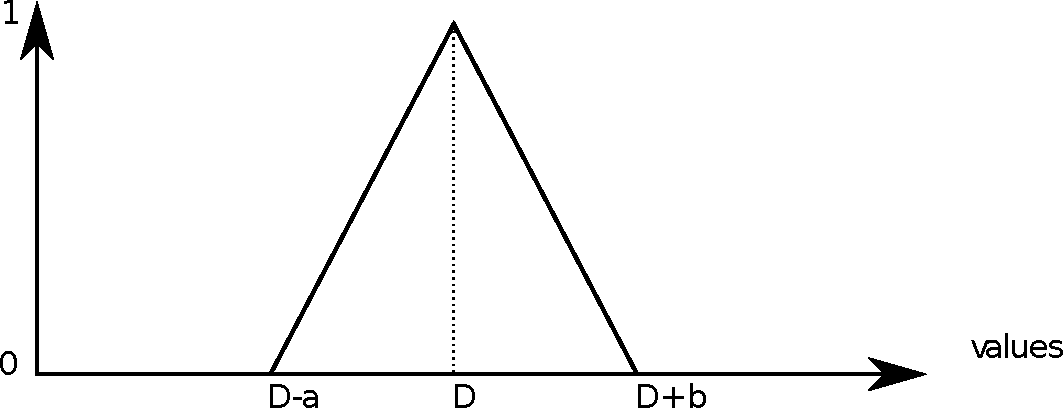
\includegraphics[scale=0.25]{./graphs/triangular.pdf}

}
\end{center}
%\centerline{ 
\psfig{file=./graphs/Y-time-point.eps}}
\vspace*{10pt}
\fcaption{\label{fig:triangular-dist}Example of fuzzy number.}
%  \label{fig:fuzzy-validity-period}
\vspace*{13pt}
\end{samepage}
If this modal value $m$ is unique, then $M$ is referred to as a \emph{fuzzy number}. 
%In other words, if the core of a fuzzy interval is a singleton, it is referred to as a fuzzy number (Figure \ref{fig:triangular-dist}).

A simple form of the membership function of a fuzzy interval is a trapezoidal function (Figure \ref{fig:trapezoidal-dist}). It can be shown that such a membership function $\mu_T$ for a fuzzy interval $T$ is convex and normalized. The values $\left[\alpha, \beta, \gamma, \delta\right]$ represent a trapezoidal possibility distribution defined by $\mu_T$:

% Four real values, denoted $\alpha$, $\beta$, $\gamma$ and $\delta$ suffice to represent a trapezoidal membership function of a fuzzy interval. In this work, a fuzzy interval defined as such will be noted as . The corresponding membership function definition for this  is then given by:

\begin{align}
\mu_T : & \quad \mathbb{R} \rightarrow \left[0,1\right] \\
\nonumber
 : & \quad x \rightarrow
\begin{cases}
1 & \mbox{ if } x \in [\beta,\gamma] \\
0 & \mbox{ if } x > \delta \vee x < \alpha \\
\frac{x-\alpha}{\beta - \alpha} & \mbox{ if } x \in [\alpha,\beta[ \\
\frac{\delta -x}{\delta - \gamma} & \mbox{ if } x \in ]\gamma,\delta] \\
\end{cases}
\end{align}

\begin{samepage}
\vspace*{13pt}
\begin{center}
{
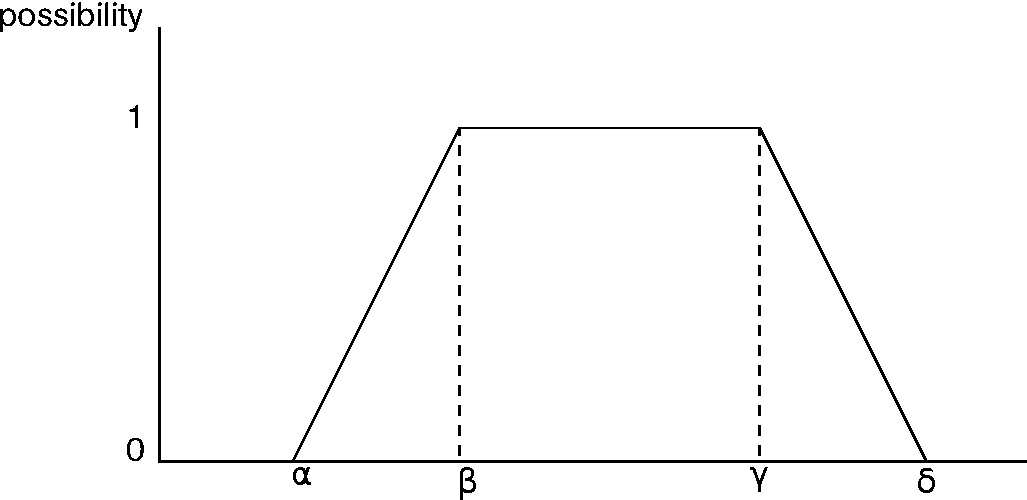
\includegraphics[scale=0.25]{./graphs/trapezoidalDistribution.pdf}

}
\end{center}
%\centerline{ 
\psfig{file=./graphs/Y-time-point.eps}}
\vspace*{10pt}
\fcaption{\label{fig:trapezoidal-dist}Example of fuzzy interval.}
%  \label{fig:fuzzy-validity-period}
\vspace*{13pt}
\end{samepage}

%\def\JPicScale{0.5}
%\begin{figure}[h!]
%  \centering
%  %%Created by jPicEdt 1.4.1_03: mixed JPIC-XML/LaTeX format
%%Thu Nov 17 17:57:10 CET 2011
%%Begin JPIC-XML
%<?xml version="1.0" standalone="yes"?>
%<jpic x-min="5" x-max="125" y-min="5" y-max="75" auto-bounding="true">
%<multicurve fill-style= "none"
%	 points= "(10,10);(10,10);(10,60);(10,60)"
%	 right-arrow= "head"
%	 />
%<multicurve fill-style= "none"
%	 points= "(10,10);(10,10);(110,10);(110,10)"
%	 right-arrow= "head"
%	 />
%<multicurve fill-style= "none"
%	 points= "(30,10);(30,10);(50,60);(50,60)"
%	 />
%<multicurve fill-style= "none"
%	 stroke-color= "#ccccff"
%	 points= "(70,60);(70,60);(90,10);(90,10)"
%	 />
%<text fill-style= "none"
%	 stroke-color= "#ff0033"
%	 stroke-width= "0.95"
%	 text-vert-align= "center-v"
%	 anchor-point= "(125,40)"
%	 text-frame= "noframe"
%	 text-hor-align= "center-h"
%	 >
%
%</text>
%<text fill-style= "none"
%	 stroke-color= "#ff0033"
%	 stroke-width= "0.95"
%	 text-vert-align= "center-v"
%	 anchor-point= "(30,5)"
%	 text-frame= "noframe"
%	 text-hor-align= "center-h"
%	 >
%$\alpha$
%</text>
%<text fill-style= "none"
%	 stroke-color= "#ff0033"
%	 stroke-width= "0.95"
%	 text-vert-align= "center-v"
%	 anchor-point= "(50,5)"
%	 text-frame= "noframe"
%	 text-hor-align= "center-h"
%	 >
%$\beta$
%</text>
%<text fill-style= "none"
%	 stroke-color= "#ff0033"
%	 stroke-width= "0.95"
%	 text-vert-align= "center-v"
%	 anchor-point= "(90,5)"
%	 text-frame= "noframe"
%	 text-hor-align= "center-h"
%	 >
%$\delta$
%</text>
%<text fill-style= "none"
%	 stroke-color= "#ff0033"
%	 stroke-width= "0.95"
%	 text-vert-align= "center-v"
%	 anchor-point= "(5,60)"
%	 text-frame= "noframe"
%	 text-hor-align= "center-h"
%	 >
%1
%</text>
%<text fill-style= "none"
%	 stroke-color= "#ff0033"
%	 stroke-width= "0.95"
%	 text-vert-align= "top"
%	 anchor-point= "(110,75)"
%	 text-rotation= "90"
%	 text-frame= "noframe"
%	 text-hor-align= "center-h"
%	 stroke-style= "dotted"
%	 >
%
%</text>
%<text fill-style= "none"
%	 text-vert-align= "center-v"
%	 anchor-point= "(45,70)"
%	 text-frame= "noframe"
%	 text-hor-align= "center-h"
%	 >
%
%</text>
%<text fill-style= "none"
%	 stroke-color= "#ff0033"
%	 stroke-width= "0.95"
%	 text-vert-align= "center-v"
%	 anchor-point= "(5,5)"
%	 text-frame= "noframe"
%	 text-hor-align= "center-h"
%	 >
%0
%</text>
%<text fill-style= "none"
%	 text-vert-align= "center-v"
%	 anchor-point= "(15,65)"
%	 text-frame= "noframe"
%	 text-hor-align= "center-h"
%	 >
%membership degree
%</text>
%<multicurve fill-style= "none"
%	 points= "(50,60);(50,60);(70,60);(70,60)"
%	 />
%<multicurve fill-style= "none"
%	 polydots-size-linewidth-scale= "2.5"
%	 polydots-style= "polydots-circle"
%	 stroke-color= "#3300cc"
%	 polydots-scale-v= "1"
%	 polydots-angle= "0"
%	 polydots-scale-h= "1"
%	 stroke-dasharray= "1;1"
%	 polydots-superimpose= "false"
%	 points= "(50,60);(50,60);(50,10);(50,10)"
%	 polydots-size-minimum= "0.7"
%	 stroke-style= "dashed"
%	 />
%<multicurve fill-style= "none"
%	 stroke-dasharray= "1;1"
%	 points= "(70,60);(70,60);(70,10);(70,10)"
%	 stroke-style= "dashed"
%	 />
%<text fill-style= "none"
%	 stroke-color= "#ff0033"
%	 stroke-width= "0.95"
%	 text-vert-align= "center-v"
%	 anchor-point= "(70,5)"
%	 text-frame= "noframe"
%	 text-hor-align= "center-h"
%	 >
%$\gamma$
%</text>
%</jpic>
%%End JPIC-XML
%LaTeX-picture environment using emulated lines and arcs
%You can rescale the whole picture (to 80% for instance) by using the command \def\JPicScale{0.8}
\ifx\JPicScale\undefined\def\JPicScale{1}\fi
\unitlength \JPicScale mm
\begin{picture}(125,75)(0,0)
\linethickness{0.3mm}
\put(10,10){\line(0,1){50}}
\put(10,60){\vector(0,1){0.12}}
\linethickness{0.3mm}
\put(10,10){\line(1,0){100}}
\put(110,10){\vector(1,0){0.12}}
\linethickness{0.3mm}
\multiput(30,10)(0.12,0.3){167}{\line(0,1){0.3}}
\linethickness{0.3mm}
\multiput(70,60)(0.12,-0.3){167}{\line(0,-1){0.3}}
\put(125,40){\makebox(0,0)[cc]{}}

\put(30,5){\makebox(0,0)[cc]{$\alpha$}}

\put(50,5){\makebox(0,0)[cc]{$\beta$}}

\put(90,5){\makebox(0,0)[cc]{$\delta$}}

\put(5,60){\makebox(0,0)[cc]{1}}

\put(110,75){\makebox(0,0)[tc]{}}

\put(45,70){\makebox(0,0)[cc]{}}

\put(5,5){\makebox(0,0)[cc]{0}}

\put(15,65){\makebox(0,0)[cc]{membership degree}}

\linethickness{0.3mm}
\put(50,60){\line(1,0){20}}
\linethickness{0.3mm}
\multiput(50,10)(0,1.96){26}{\line(0,1){0.98}}
\linethickness{0.3mm}
\multiput(70,10)(0,1.96){26}{\line(0,1){0.98}}
\put(70,5){\makebox(0,0)[cc]{$\gamma$}}

\end{picture}

%  \caption{Trapezoidal membership function}
%  \label{fig:trapezoidal}
%\end{figure}


The representation for a triangular possibility distribution is given by three values $\left[D,a,b \right]$. The distribution is obtained from a trapezoidal possibility distribution by replacing the values $\left[D-a, D, D, D+b \right]$.


% The most convenient form of the membership function of a fuzzy number is a triangular form. It can be shown that such a membership function $\mu_M$ for a fuzzy number $M$ is convex and normalized. Three real values, denoted by $a$, $b$ and $D$, suffice to represent a triangular membership function of a fuzzy number and in this work, a fuzzy number defined as such will be noted as $\left[D, a, b \right]$. Here:
% \begin{itemize}
% \item
% $D$ denotes the single value in the core of $M$
% \item
% $D-a$ is then $\inf \{u \in \mathbb{R} : \mu_{M}(u) > 0\}$
% \item
% $D+b$ is then $\sup \{u \in \mathbb{R} : \mu_{M}(u) > 0\}$
% \end{itemize}
% 
% The membership function of such a fuzzy number is then given by:
% 
% \vspace{-10pt}
% 
% \begin{align}
% \mu_M :   \mathbb{R} \rightarrow \left[0,1\right] :  x \rightarrow \nonumber\\
% \begin{cases}
% \nonumber
% 0 & \mbox{ if } \left(x < D-a\right) \vee \left(x > D+b\right) \\
% \frac{\left[x-\left(D-a\right)\right]}{a} & \mbox{ if } \left(x \geq D-a\right) \wedge (x \leq D)  \\
% -\frac{\left[x-\left(D+b\right)\right]}{b} & \mbox{ if } \left(x \geq D\right) \wedge (x \leq D+b)
% \end{cases}
% \end{align}

%\begin{figure}[h!]
%  \centering
%  %%Created by jPicEdt 1.4.1_03: mixed JPIC-XML/LaTeX format
%%Thu Jan 12 17:26:56 CET 2012
%%Begin JPIC-XML
%<?xml version="1.0" standalone="yes"?>
%<jpic x-min="-2.5" x-max="60" y-min="-2" y-max="32.5" auto-bounding="true">
%<multicurve right-arrow= "head"
%	 fill-style= "none"
%	 points= "(0,0);(0,0);(55,0);(55,0)"
%	 />
%<multicurve right-arrow= "head"
%	 fill-style= "none"
%	 points= "(0,0);(0,0);(0,30);(0,30)"
%	 />
%<text right-arrow= "head"
%	 fill-style= "none"
%	 text-vert-align= "center-v"
%	 anchor-point= "(-2.5,27.5)"
%	 text-frame= "noframe"
%	 text-hor-align= "center-h"
%	 >
%1
%</text>
%<text right-arrow= "head"
%	 fill-style= "none"
%	 text-vert-align= "center-v"
%	 anchor-point= "(-2.5,0)"
%	 text-frame= "noframe"
%	 text-hor-align= "center-h"
%	 >
%0
%</text>
%<text right-arrow= "head"
%	 fill-style= "none"
%	 text-vert-align= "center-v"
%	 anchor-point= "(15,32.5)"
%	 text-rotation= "135"
%	 text-frame= "noframe"
%	 text-hor-align= "center-h"
%	 >
%Membership Degree
%</text>
%<multicurve fill-style= "none"
%	 points= "(4,0);(4,0);(15,27.5);(15,27.5)"
%	 />
%<multicurve fill-style= "none"
%	 points= "(15,27.5);(15,27.5);(42,0);(42,0)"
%	 />
%<text fill-style= "none"
%	 text-vert-align= "center-v"
%	 anchor-point= "(60,0)"
%	 text-frame= "noframe"
%	 text-hor-align= "center-h"
%	 >
%Time
%</text>
%<text fill-style= "none"
%	 text-vert-align= "center-v"
%	 anchor-point= "(16,-2)"
%	 text-frame= "noframe"
%	 text-hor-align= "center-h"
%	 >
%$D$
%</text>
%<text fill-style= "none"
%	 text-vert-align= "center-v"
%	 anchor-point= "(4,-2)"
%	 text-frame= "noframe"
%	 text-hor-align= "center-h"
%	 >
%$D-a$
%</text>
%<text fill-style= "none"
%	 text-vert-align= "center-v"
%	 anchor-point= "(42,-2)"
%	 text-frame= "noframe"
%	 text-hor-align= "center-h"
%	 >
%$D+b$
%</text>
%</jpic>
%%End JPIC-XML
%LaTeX-picture environment using emulated lines and arcs
%You can rescale the whole picture (to 80% for instance) by using the command \def\JPicScale{0.8}
\ifx\JPicScale\undefined\def\JPicScale{1}\fi
\unitlength \JPicScale mm
\begin{picture}(60,32.5)(0,0)
\linethickness{0.3mm}
\put(0,0){\line(1,0){55}}
\put(55,0){\vector(1,0){0.12}}
\linethickness{0.3mm}
\put(0,0){\line(0,1){30}}
\put(0,30){\vector(0,1){0.12}}
\put(-2.5,27.5){\makebox(0,0)[cc]{1}}

\put(-2.5,0){\makebox(0,0)[cc]{0}}

\put(15,32.5){\makebox(0,0)[cc]{Membership Degree}}

\linethickness{0.3mm}
\multiput(4,0)(0.12,0.3){92}{\line(0,1){0.3}}
\linethickness{0.3mm}
\multiput(15,27.5)(0.12,-0.12){225}{\line(0,-1){0.12}}
\put(60,0){\makebox(0,0)[cc]{Time}}

\put(16,-2){\makebox(0,0)[cc]{$D$}}

\put(4,-2){\makebox(0,0)[cc]{$D-a$}}

\put(42,-2){\makebox(0,0)[cc]{$D+b$}}

\end{picture}

%  \caption{Triangular membership function.}
%  \label{fig:triangular}
%\end{figure}



\subsection{\label{subsec:interval-evaluation-by-ill-known-constraints}Interval Evaluation by Ill-known Constraints}
In our case, we need to know if all points in a crisp interval $I$ reside between the boundaries of an ill-known interval $\left[ X , Y \right]$. To compute that, we introduce the concept of \emph{ill-known constraint}\cite{Pons2011}.




\begin{definition}
Given a universe $U$, an ill-known constraint $C$ on a set $A \subseteq U$ is specified by means of a binary relation $R \subseteq U^{2}$ and a fixed ill-known value denoted by its possibilistic variable $V$ over $U$, i.e.:
\begin{align}
\label{eq:ill-known-constraint}
C \triangleq (R,V)
\end{align}
Set $A$ satisfies the constraint if and only if:
\begin{align}
\forall a \in A : (a,V) \in R
\end{align}
\end{definition}

An example of an ill-known constraint is $C_{ex} = (<, X)$. Some set $A$ satisfies $C_{ex}$ if $\forall a \in A : a < X$, given the possibilistic variable $X$.

The satisfaction of a constraint $C \triangleq (R,V)$ by a set $A$ is still a Boolean matter, but due to the uncertainty about the ill-known value $V$, it can be uncertain whether $C$ is satisfied by $A$ or not \cite{Pons2011}. In fact, this satisfaction now behaves as a proposition. Based on the possibility distribution $\pi_{V}$ of $V$, the possibility and necessity that $A$ satisfies $C$ can be computed. This proposition can thus be seen as a possibilistic variable on $\mathbb{B}$. The required possibility and necessity are:

\vspace{-10pt}

\begin{align}
\label{ill-known-pos}\
\Pos(A\text{ satisfies }C) & =\\
\nonumber
\min_{a \in A}\left(\sup_{(a,w) \in R}\pi_{V}(w)\right) \\
\label{ill-known-nec}
\Nec(A\text{ satisfies }C) & =\\
\nonumber
\min_{a \in A}\left(\inf_{(a,w) \notin R} 1-\pi_{V}(w)\right) 
\end{align}

So far, we have shown how it can be verified whether a set satisfies or not an ill-known constraint. The interval evaluation problem is explained in a more general context in \cite{Pons2011}.

\begin{samepage}
\vspace*{13pt}
\begin{center}
{
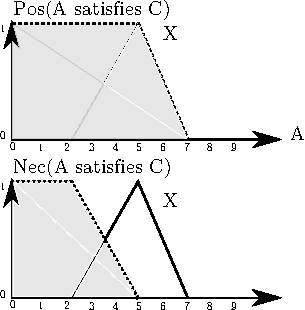
\includegraphics[scale=1]{./graphs/example-ill-known.pdf}
}
\end{center}
%\centerline{ 
\psfig{file=./graphs/Y-time-point.eps}}
\vspace*{10pt}
\fcaption{\label{fig:example-ill-known}Example of the evaluation of the ill-known constraint $C \triangleq (\leq, X), X = \left[5, 3, 2\right]$. Possibility and necessity measures are shown in grey. }
%  \label{fig:fuzzy-validity-period}
\vspace*{13pt}
\end{samepage}


\begin{example}
Consider  $X = \left[5, 3, 2 \right]$ and let $C =(\leq, X)$ the ill-known constraint. Then, the evaluation of the possibility and the necessity are obtained from \eqref{ill-known-pos} and \eqref{ill-known-nec} respectively. (See Figure \ref{fig:example-ill-known}).






 
\begin{align}
\Pos(A\text{ satisfies }C) & =\\
\nonumber
\min_{a \in A}\left(\sup_{a \leq w}\pi_{X}(w)\right)\\
\Nec(A\text{ satisfies }C) & =\\
\nonumber
\min_{a \in A}\left(\inf_{a > w} 1-\pi_{X}(w)\right) 
\end{align}




\end{example}





It is observed that Boolean combinations of constraints are required. For example, the problem of interval evaluation (explained earlier) requires that all the elements of an interval $[a,b]$ are larger than a value $X$ and, at the same time, smaller than a value $Y$, which implies that a conjunctive Boolean combination of both constraints must be satisfied. To allow Boolean combinations of constraints, the following definitions are introduced.
\begin{definition}
\label{def:set-evaluation}
Consider a universe $U$, an $n$-ary vector $\mathbf{C}$ of constraints and a Boolean function $\bool:\mathbb{B}^{n}\rightarrow\mathbb{B}$. An evaluation function is defined by:
\begin{equation}
\lambda:\Pow(U)\rightarrow\mathbb{B}:\lambda(A)\mapsto\bool\Big(C_{1}(A),...,C_{n}(A)\Big).
\end{equation}
\end{definition}
Definition \ref{def:set-evaluation} presents a function that evaluates a Boolean combination of some basic constraints. Informally, it states that a set $A$ passes the evaluation made by $\lambda$ if the Boolean combination of some propositions equals $T$. This crisp definition can be generalized to the case of ill-known constraints.
\begin{definition}
\label{def:ill-known-sets}
Consider a universe $U$, an $n$-ary vector $\mathbf{C}$ of ill-known constraints and a Boolean function $\bool:\mathbb{B}^{n}\rightarrow\mathbb{B}$. The uncertainty about the evaluation of a set $A$ by an evaluation function $\lambda$ is then given by:
\begin{equation}
\forall A\in\Pow(U):\pi_{\lambda(A)}=\widetilde{\bool}\Big(\pi_{C_1(A)},...,\pi_{C_n(A)}\Big)\\
\end{equation}
Hereby, $\widetilde{\bool}$ is the possibilistic extension of $\bool$.
\end{definition}
It is well known that any Boolean function $\bool$ can be cast to a canonical form~\cite{McCluskey1965}, requiring only logical conjunction $\wedge$, logical disjunction $\vee$ and logical negation. Therefore, only those connectives will be treated within the scope of this paper. By applying the possibilistic extensions of $\wedge$, $\vee$ and $\neg$, concrete equations are obtained for the calculations of uncertainty about the evaluation of a set by means of an evaluation function $\lambda$. In the case of conjunction (i.e., $\bool=\wedge$), the inference of uncertainty about the evaluation of a set reduces to:
\begin{eqnarray}
\label{eq:conjunctive1}
\forall A\in\Pow(U):\Pos(\lambda(A))&=\\
\nonumber
\min_{i=1 \ldots n}\Pos\left(C_i(A)\right)\\
\label{eq:conjunctive2}
\forall A\in\Pow(U):\Nec(\lambda(A))&=\\
\nonumber
\min_{i=1 \ldots n}\Nec\left(C_i(A)\right).
\end{eqnarray}
In the case of disjunction (i.e. $\bool=\vee$), the inference of uncertainty about the evaluation of a set reduces to:
\begin{eqnarray}
\label{eq:disjunctive}
\forall A\in\Pow(U):\Pos(\lambda(A))&=\\
\nonumber
\max_{i=1 \ldots n}\Pos\left(C_i(A)\right)\\
\forall A\in\Pow(U):\Nec(\lambda(A))&=\\
\nonumber
\max_{i=1 \ldots n}\Nec\left(C_i(A)\right).
\end{eqnarray}
Note that by using the functions $\min$ and $\max$ here, there is an implicit assumption that the possibilistic variables $\pi_{C_i}$ are mutual $\min$-dependent in the sense of De Cooman (i.e. non-interactive). For an extensive reading on (in)dependency of possibilistic variables, the reader is referred to~\cite{GertDeCooman1997b},\cite{GertDeCooman1997a},\cite{GertDeCooman1997}. In case of $\neg$, we get:
\begin{eqnarray}
\label{eq:negation}
\forall A\in\Pow(U):\Pos(\neg\lambda(A))&=\\
\nonumber
1-\Nec(\lambda(A))\\
\forall A\in\Pow(U):\Nec(\neg\lambda(A))&=\\
\nonumber
1-\Pos(\lambda(A)).
\end{eqnarray}

\begin{example}
Consider that we want to check if the crisp interval $I = \left[j, k\right]$ is included in $\left[X, Y\right]$. In this situation, two ill-known constraints are constructed.

%We assume that $X$ specifies the lower bound and $Y$ the upper bound for a given interval, we want to known whether all points in the interval are larger than or equal to $X$ and smaller than or equal to $Y$. Therefore, we consider two ill-known constraints:

\vspace{-10pt}

\begin{eqnarray}
\label{eq:constraint-c1}
C_1 & \triangleq\left(\geq,X\right)\\
\label{eq:constraint-c2}
C_2 & \triangleq\left(\leq,Y\right)
\end{eqnarray}

To calculate the possibility and necessity concerning a conjunction of constraints, the $\min$ operator can be used. The possibility and necessity of $I$ being included in $\left[X, Y\right]$ are now: %satisfying both constraints is then:

\vspace{-10pt}

\begin{align}
\label{eq:interval-pos}
\Pos(I\text{ satisfies }C_1\ and\ C_2) & =\\
\nonumber
\min_{a \in I}\left(\sup_{a \geq w}\pi_{X}(w),\sup_{a \leq v}\pi_{Y}(v)\right)\\
\label{eq:interval-nec}
\Nec(I\text{ satisfies }C_1\ and\ C_2) & =\\
\nonumber
\min_{a \in I}\left(\inf_{a < w} 1-\pi_{X}(w),\inf_{a > v} 1-\pi_{Y}(v)\right).
\end{align}
\end{example}

There is a special boolean combination of constraints that is of particular interest; let us see it.
\begin{definition}
\emph{Conjunctive combination of ill-known constraints}. Consider a universe $U$. Let $R_1, R_2$ be two binary relations in U. Let $X_1, X_2$ be two fixed ill-known values in $U$. Let  $C_1 = (R_1, X_1)$ and $C_2 = (R_2, X_2)$ be two ill-known constraints. A conjunctive combination of both constraints is given by:
\begin{align}
\label{eq:convex-combination}
CC \triangleq \left \lbrace C_1 \wedge C_2 \right \rbrace
\end{align}
In a more general way, it is possible to define the conjunctive combination of an n-ary vector of constraints:
\begin{align}
\label{eq:nary-convex-combination}
CC \triangleq \left \lbrace C_1 \wedge \ldots \wedge C_n \right \rbrace
\end{align}
\end{definition}

\begin{theorem}
\label{th:convex-combination-ill-known-constraints}
Consider the conjunctive combination $CC$ of any n-ary vector $\left \lbrace C_{1_{Z_1}}, \ldots, C_{n_{Z_n}} \right \rbrace$ of constraints over the ill-known variables $Z_1, \ldots, Z_n$. Then, if $\pi_{C_1(Z_1)}, \ldots, \pi_{C_n(Z_n)}$ are convex, then  $\pi_{CC}$ is also convex.
\end{theorem}

\begin{proof}
Let $CC \triangleq \left \lbrace C_{1_{Z_1}} \wedge \ldots \wedge C_{n_{Z_n}}  \right \rbrace$. Then:
\begin{align}
\label{eq:proof-convex1}
\pi_{CC} \left( \lambda x_1 + \left( 1 - \lambda \right)x_2 \right) = \\
\nonumber
\min  \big( \pi_{C_1(Z_1)}\left( \lambda x_1 + \left( 1 - \lambda \right)x_2 \right), \ldots,\\
\nonumber
   \pi_{C_n(Z_n)}\left( \lambda x_1 + \left( 1 - \lambda \right)x_2 \right)  \big)
\end{align}
Since $\pi_{C_1(Z_1)}, \ldots, \pi_{C_n(Z_n)}$ are convex:
\begin{align}
\label{eq:proof-convex2}
\pi_{C_1(Z_1)} \left(\lambda x_1 + \left( 1 - \lambda \right)x_2  \right) \geqq \\
\nonumber
\min \big(\pi_{C_1(Z_1)} \left( x_1 \right),\pi_{C_1(Z_1)} \left( x_2 \right)  \big)\\
\nonumber
\vdots \\
\nonumber
\pi_{C_n(Z_n)} \left(\lambda x_1 + \left( 1 - \lambda \right)x_2  \right) \geqq \\
\nonumber
\min \big(\pi_{C_n(Z_n)} \left( x_1 \right),\pi_{C_n(Z_n)} \left( x_2 \right) \big) 
\end{align}
Then, by using equation \eqref{eq:proof-convex1}:
\begin{align}
\label{eq:proof-convex3}
\pi_{CC} \left( \lambda x_1 + \left( 1 - \lambda \right)x_2 \right) \geqq  \\
\nonumber
\min \big( \min \left(\pi_{C_1(Z_1)} \left( x_1 \right),\pi_{C_1(Z_1)} \left( x_2 \right) \right),\\
\nonumber
\ldots, \min \left(\pi_{C_n(Z_n)} \left( x_1 \right),\pi_{C_n(Z_n)} \left( x_2 \right) \right) \big)
\end{align}
Which is equivalent to the following:
\begin{align}
\label{eq:proof-convex4}
\pi_{CC} \left( \lambda x_1 + \left( 1 - \lambda \right)x_2 \right) \geqq  \\
\nonumber
\min \big( \min \left(\pi_{C_1(Z_1)} \left( x_1 \right), \ldots, \pi_{C_n(Z_n)} \left( x_1 \right) \right),\\
\nonumber
\ldots, \min \left(\pi_{C_1(Z_1)} \left( x_2 \right), \ldots, \pi_{C_n(Z_n)} \left( x_2 \right) \right) \big)
\end{align}
Finally we obtain:
\begin{align}
\label{eq:proof-convex5}
\pi_{CC} \left( \lambda x_1 + \left( 1 - \lambda \right)x_2 \right) \geqq  \\
\nonumber
\min \big(\pi_{CC} \left( x_1 \right), \pi_{CC} \left( x_2 \right) \big)
\end{align}
\end{proof}

Sometimes, an ill-known value might be specified by a convex combination of ill-known constraints. This allow to define ill-known values by means of relationships with respect to other ill-known points.

%\begin{definition}
%\emph{Ill-known point defined by ill-known constraints}
%Consider a universe $U$, an n-ary vector $\mathbf{C}$ of ill-known constraints and a Boolean function $\bool:\mathbb{B}^{n}\rightarrow\mathbb{B}$. An ill-known value $X$ is defined by:
%\begin{align}
%\label{eq:ill-known-value-def-by-const}
%X \in \Pow(U):\pi_{X}=\widetilde{\bool}\Big(\pi_{C_1(Z_1)},...,\pi_{C_n(Z_n)}\Big)\\
%\end{align} 
%\end{definition}

\begin{definition}
\label{def:convex-combination-ill-known-constraints}
\emph{Ill-known value defined by conjunctive combination of constraints.}
Consider a universe $U$, $CC \triangleq \left \lbrace C_{1_{Z_1}} \wedge \ldots \wedge C_{n_{Z_n}}  \right \rbrace$ a conjunctive combination of ill-known constraints over the variables $Z_1, \ldots, Z_n$. The uncertainty about the evaluation of an ill-known value $X$ is given by:
\begin{align}
\label{eq:ill-known-value-def-by-const-unc}
X \in \Pow(U):\pi_{X}=\pi_{CC}
\end{align} 

The definition of the ill-known value $X$ with respect to the conjunctive combination of ill-known constraints, is written as:
\begin{align}
\label{eq:ill-known-value-by-convex-constraints}
X \triangleq CC 
\end{align}


Note that $\pi_{X}$ is convex since $\pi_{CC}$ is convex as demonstrated in Theorem \ref{th:convex-combination-ill-known-constraints}.
\end{definition}


\begin{example}
As an example, consider the hospital database. When a patient enters o leaves a medical service in hospital, a record tracking the patient is stored. The exact time for this is not precisely known. Consider now that $X = \left[12, 2, 2\right]$ is the time in hours when a patient left the emergency service and $Y = \left[18, 2, 1 \right]$ is the time in hours when the patient left the hospital. It is possible to obtain $Z$ (the period of time between the emergency service and the left of the patient) by using a conjunctive combination of constraints.

\begin{align}
\nonumber
CC = \left \lbrace C_1\left(>,X\right) \wedge C_2(\leq,Y) \right \rbrace \\
\nonumber
Z = CC
\end{align}
$Z$ is a fuzzy interval defined by a trapezoidal shape given by $\left[12,\ 14,\ 18,\ 19 \right]$.
Figure \ref{fig:example-ill-known-by-const} illustrates the relations among the variables $X$, $Y$ and $Z$.
\end{example}

\begin{samepage}
\vspace*{13pt}
\begin{center}
{
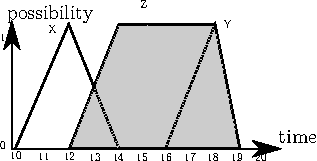
\includegraphics[scale=1]{./graphs/ill-known-by-constraints.pdf}

}
\end{center}
%\centerline{ 
\psfig{file=./graphs/Y-time-point.eps}}
\vspace*{10pt}
\fcaption{\label{fig:example-ill-known-by-const}Ill-known values $X$ and $Y$. The grey area represents the ill-known value $Z$ defined by the convex combination of the two ill-known constraints $C_1$ and $C_2$.}
\vspace*{13pt}
\end{samepage}

%\paragraph{Example} Consider the ill-known values $X = \left[5, 2, 8\right]$ and $Y = \left[9, 7, 10 \right]$. The knowledge about the evaluation of the interval $\left[a, b \right]$  is given by the expressions \eqref{eq:interval-pos},\eqref{eq:interval-nec}.  Figure~\ref{fig:3d-possibility} shows a 3D plot of the possibility that an interval $[a,b]$ passes the evaluations specified by the ill-known constraints. Note the triangular form for the resulting possibility distribution since the condition $a \leq b$ holds.
%
%\begin{figure}[h!]
%\centering
%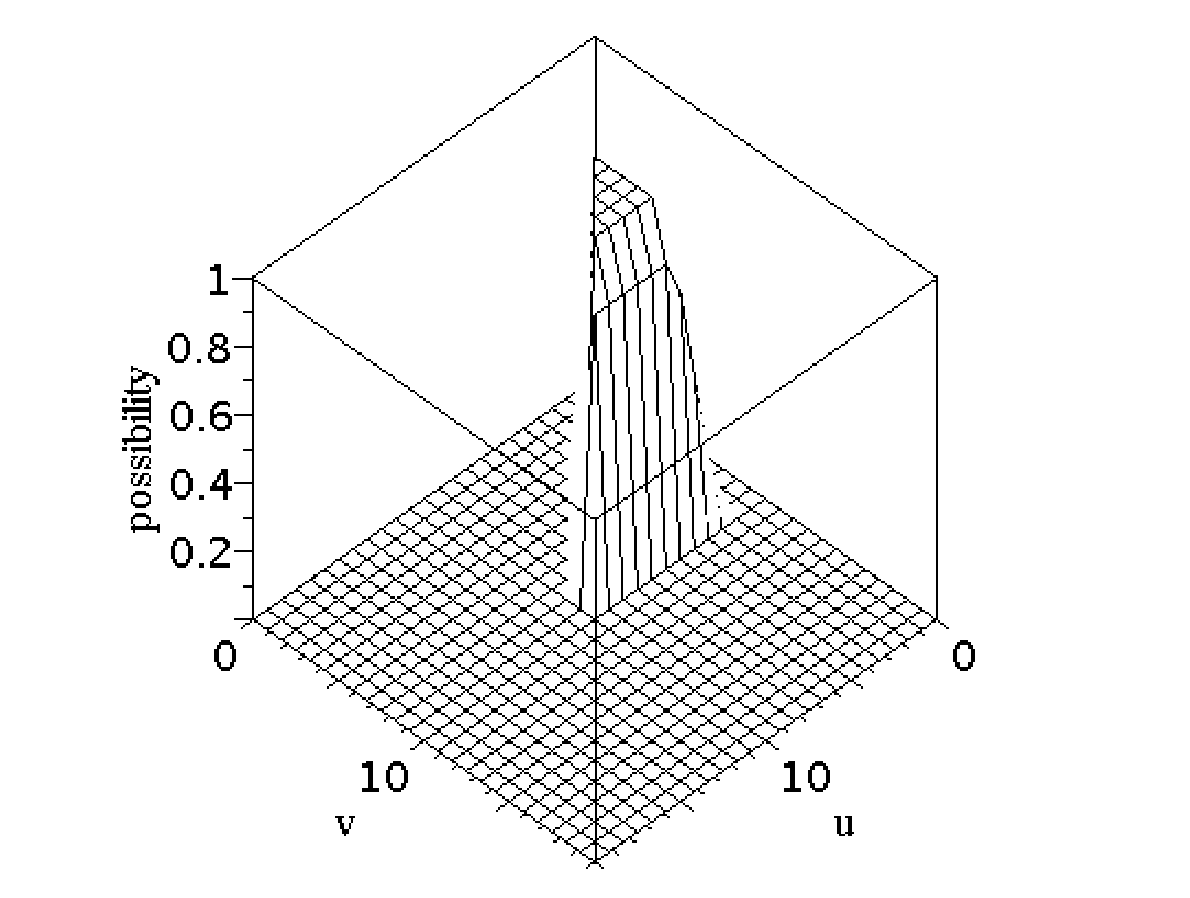
\includegraphics[scale=0.4]{graphs/3D_possibility.eps}
%\caption{Possibility of evaluation for the interval $[a,b]$.}
%\label{fig:3d-possibility}
%\end{figure}
%The necessity plot is obtained in a similar way and is shown in Figure~\ref{fig:3d-necessity}. Notice that the necessity measure is not normalized because the supports of $X$ and $Y$ overlap.
%\begin{figure}[h!]
%\centering
%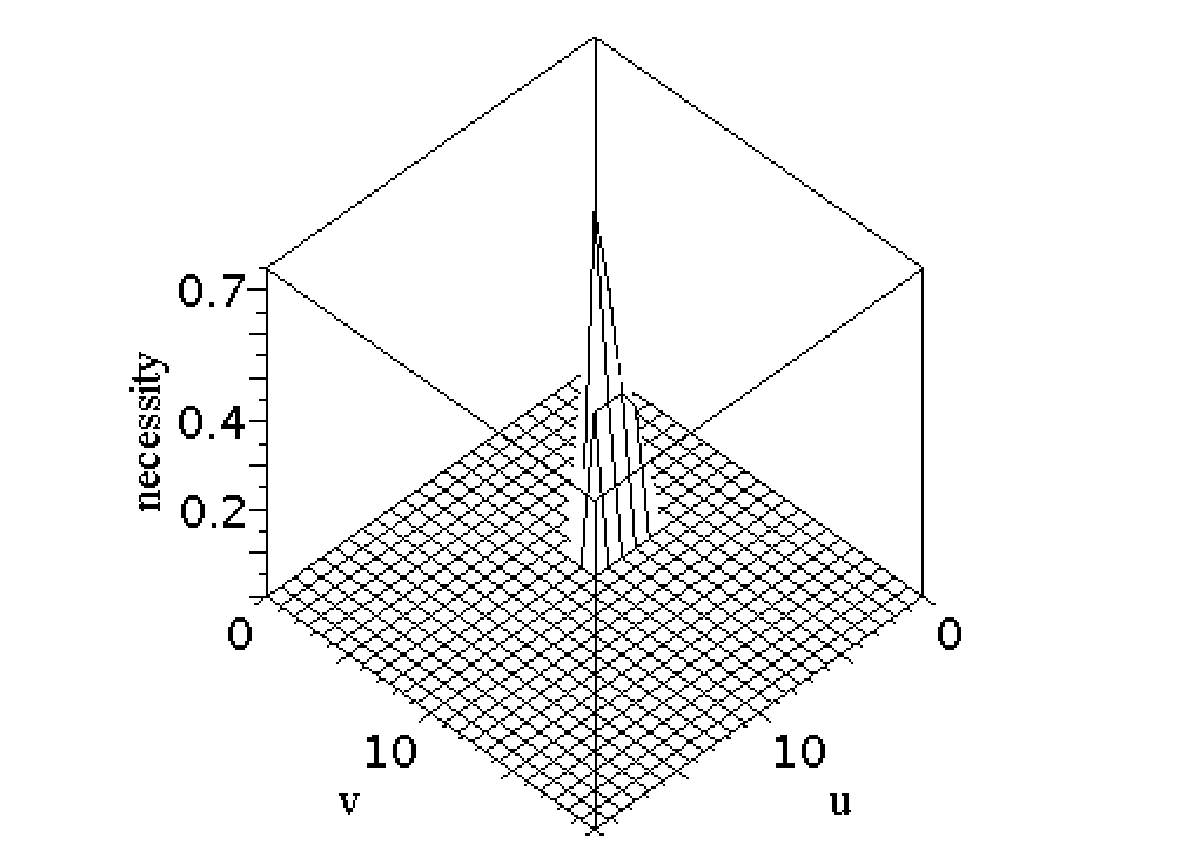
\includegraphics[scale=0.4]{graphs/3D_necessity.eps}
%\caption{Necessity of evaluation for the interval $[a,b]$.}
%\label{fig:3d-necessity}
%\end{figure}

%enlace:
We have seen the main theoretical concepts about ill-known values. Now, we are going to explain the main concepts about the treatment of time and the imperfection related to the time in databases. This two preliminary analysis will be the pillars of our proposal in section \ref{sec:time-rep}.

%In the following subsections we will show how to represent imperfect time intervals by means of ill-known values.



%%%%%%%%%%%%%%%%%%%%%%%%%%%%%%%%%%%%%%%%%%%%%%%%%%%%%%%%%%%%%%%%%%%%%%%%%
%
% Time
%
%%%%%%%%%%%%%%%%%%%%%%%%%%%%%%%%%%%%%%%%%%%%%%%%%%%%%%%%%%%%%%%%%%%%%%%%%
\subsection{\label{subsec:time-in-databases}Time in Databases}
The concept of time has been studied in databases for a long time. A true standard for adding temporal aspects to relational databases does not exist, but there is a consensus in the literature \cite{Dyreson1994} on what is called a \emph{temporal database}: a temporal database is a database dealing with some aspects of time in its schema.
In a temporal DBMS, a \textbf{chronon} is the shortest duration of time supported by the system. In temporal databases, some temporal attributes can be managed without treating the attribute differently from non-temporal attributes. The time described by such an attribute is called \textbf{user defined time} (\emph{UDT}). In addition to UDT, the following types of time can be discerned in a temporal database, all of which are handled exceptionally by the DBMS:

\begin{itemize}
	\item
	\textbf{Transaction time} (\emph{TT}) \cite{Rowe1987},\cite{Jensen1991} denotes the time when the fact (object) is stored in the database. It is usually append-only: as the past can not be changed, TT can not be changed neither. Furthermore, at the moment of insertion, a TT can be neither in the past nor in the future.
	\item
	\textbf{Valid time} (\emph{VT}) \cite{Jensen1994},\cite{Sarda1990},\cite{McKenzie1981} denotes the time when the fact (object) is true in the modelled reality. A fuzzy extension has been proposed by \cite{Garrido2009}. 
%	\item
%	User defined time: It is an uninterpreted attribute. The domain is date/time. The query language has no special support for it.
	\item
	\textbf{Decision time} (\emph{DT}) \cite{Nascimento1995},\cite{Chakravarthy1994},\cite{Etzion1992},\cite{Ozsoyoglu1995} denotes the time when an event was decided to happen. 
	\end{itemize}
	
	E.g., consider a database containing employee contract descriptions. The time when the employee's contract is valid, represented by an interval, is VT. The time when the employee's contract is stored in the database is the TT. The time when the decision for hiring this employee was made is the DT.

% is a non-decomposable unit of time.  it  There are two ways to represent a chronon: as a point or as an interval \cite{655777}.

When working with these time concepts, the Data Manipulation Language (\emph{DML}, which is part of the standard database querying language SQL) is extended to deal with possible temporal inconsistencies within the data and to handle more complex (temporal) queries. 
%Next to these concepts, also \textbf{user defined time} (\emph{UDT}) is discerned. UDT is an uninterpreted attribute in the date/time domain. This means that the attribute uses the date/time domain, but the database model does not treat the attribute differently from non-temporal attributes.
Depending on the time managed, a database is classified as either a \textbf{Valid Time Database} (\emph{VTDB}), a \textbf{Transaction Time Database} (\emph{TTDB}), a \textbf{bi-temporal database} (both valid and transaction time are managed) or a \textbf{tri-temporal} or \emph{multitemporal} database (valid time, transaction time and decision time are managed).

%\subsection{Temporal Elements}
%%	
%	In order to define a temporal database model, some basic elements should be defined \cite{Dyreson:1994:CGT:181550.181560}:
%	\begin{itemize}
%	\item A	\textbf{chronon} is a non-decomposable unit of time. In a temporal DBMS, it is the shortest duration of time supported by the system. There are two ways to represent a chronon: as a point or as an interval \cite{655777}.
%	\item
%	\emph{Event}: An instant of time. Usually, an event is said to be occur during time $t$ if it occurs during the chronon represented by $t$.
%	\item
%	\emph{Interval}: The time between two events. The representation is very often a set of contiguous chronons.
	%\item
	%\emph{Span}: A directed duration of time. A duration is an amount of time with known  lenght but no specific starting or ending chronons. The span can be either positive, denoting a forward motion of time or negative, denoting a backward motion of time.
%	\item A	\textbf{timestamp} is a time value associated with some object in the database.	
	
%	\item The	\textbf{lifespan} (of a database object)is the time over which it is defined. The lifespan of a valid time object denotes the time when the corresponding object exists. The lifespan of a transaction time object is the value of the timestamp.
	
	
	
	
	
%	Depending on the type of time the meaning is different:
%		\begin{itemize}
%		\item
%		Lifespan of a valid time object: Refers the time when the corresponding object exists.	
%		\item
%		Lifespan of a transaction time object: The transaction time of a database object refers when the object is stored in the database. The lifespan is the value of the timestamp.		
%		\end{itemize}
%	\end{itemize}
	
%	In the temporal database thesaurus, \emph{'Snapshot'} is the word for non-temporal matters. As a temporal database is a generalization for relational databases, an \emph{snapshot database} is a relational database. Furthermore, a \emph{snapshot relation} is a relation incorporating neither valid nor transaction time.

%\subsection{Main issues when dealing with time}
%Among others, the following problems are present when dealing with time in a database:

%	\begin{itemize}	
%	\item \textbf{Granularity} denotes a partition on the set of chronons. The conversion between several granularities is studied in \cite{Lin97efficientconversion}. Granularity is the base of the temporal model in \cite{Cru97}. An object-oriented implementation is in \cite{624013}.
%	\item	To ensure \textbf{consistency}, temporal databases usually redefine the primary key of a relation. The new primary key takes into account the presence of the time. In order to keep the consistency, the DML is re-defined. For example, in a VTDB, the temporal update sentence is usually composed by an update sentence (closing the old row) plus an insert sentence (creating the new row).
%	\end{itemize}
%Guy's suggestion: instead of imprecision, use imperfection which is more general.
\subsubsection{Imperfection and time}
Representing imprecision and its semantics when dealing with time has been studied for a long time. Several proposals for representing and computing imprecise time indications can be found in \cite{DeCaluwe1997} and \cite{DeTre1997}. Also, the changes between several granularities can be seen as a source of imprecision \cite{Devos1998}.

In the proposal section we will consider two kinds of imprecision:
\begin{itemize}
\item \textbf{Uncertainty in the database} denotes the uncertainty that arises when the knowledge about the temporal data in the database is uncertain. E.g., a database record shows that \emph{`The car is in the garage around April.'}
 \item \textbf{Imprecision in the query specification} denotes the imprecision in the specification of temporal criteria by the user, when querying. E.g., \emph{`The user wants to obtain a car which is red and which is in the garage around April.'}
\end{itemize}

\subsubsection{Representation}
Several proposals for managing uncertain time in a database exist. Some proposals work with rough sets \cite{Qiang2009}, other proposals rely on possibility distributions for representing uncertainty in time \cite{Dyreson1998},\cite{Garrido2009}, \cite{Galindo2001}. In order to compare temporal possibility distributions, extensions of the classical Allen's operators \cite{Allen1983} are defined in \cite{Ohlbach2004}, \cite{Nagypal2003},\cite{Dubois2003a} and \cite{Schockaert2008}
%In the proposal section, we will follow the representation by means of possibility distributions, in order to work with both satisfaction and dissatisfaction degrees. Also, in order to work properly with fuzzy operators, the underlying domain should be numeric. 
% Take a look into this:
%In this paper, the representation for the dates will follow the Julian Day Number (JDN) representation \cite{Dir96}.

%If the starting points and/or the end points of the interval representing the time are not known precisely, it is easy to fuzzify them, using, e.g., two triangular possibility distributions.


In order to deal with uncertainty in time intervals, several proposals are made. Here, two approaches are introduced: the first one, based on \emph{Fuzzy Validity Period}~\cite{Garrido2009} and the second one based on \emph{Possibilistic Valid-time Period}~\cite{JoseEnriquePons2012}.

\begin{definition}
A \textbf{Fuzzy Validity Period} (\emph{FVP}) is defined as a fuzzy time interval specifying when an object is valid. A fuzzy time interval is then the fuzzification of a crisp time interval.
\end{definition}
Several options to transform possibility distributions corresponding to the fuzzy starting point and the fuzzy end point into one consistent FVP exist \cite{Garrido2009}, e.g (Fig. \ref{fig:fuzzy-validity-period}):
\begin{itemize}
\item The \textbf{convex hull} approach is the most intuitive approach. The resulting FVP is the convex hull of the union of both fuzzy sets.
\item The \textbf{uncertainty preserving} approach is less intuitive but more realistic. The amount of uncertainty is maintained at the edges of the possibility distribution representing the FVP \cite{Garrido2009}.
\end{itemize}

%%%%%%
% FUZZY VALIDITY PERIOD
%%%%%%
\vspace*{13pt}
\begin{center}
{
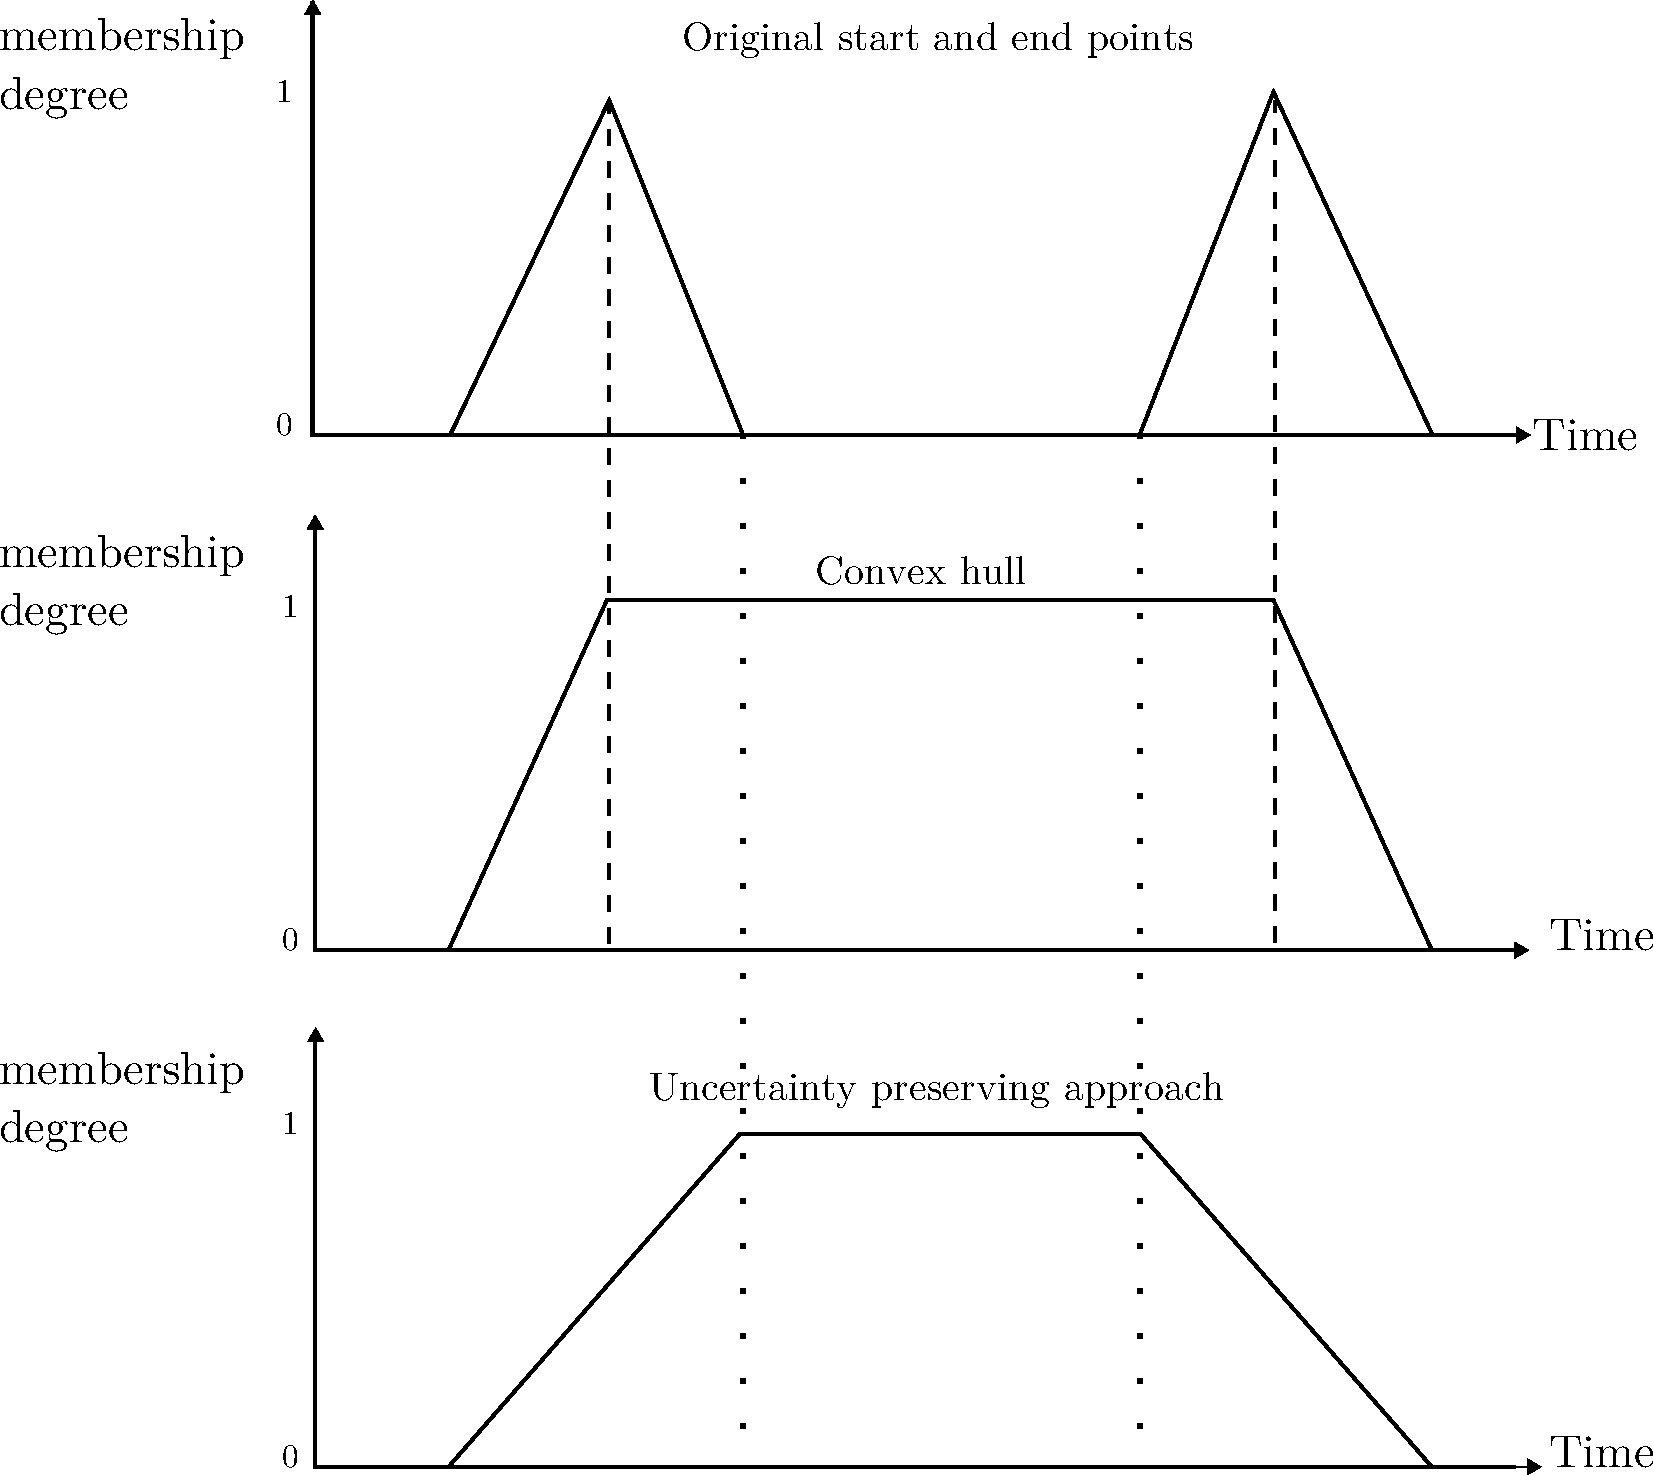
\includegraphics[scale=0.25]{./graphs/comparisoncv.pdf}

}
\end{center}
%\centerline{ 
\psfig{file=./graphs/Y-time-point.eps}}
\vspace*{10pt}
\fcaption{\label{fig:fuzzy-validity-period}Transformation to obtain the FVP. The top graph shows the two triangular possibility distributions. The middle graph shows the convex hull validity period, the bottom one shows the result of the second transformation, which maintains the imprecision.}
%  \label{fig:fuzzy-validity-period}
\vspace*{13pt}

\begin{definition}
A \textbf{Possibilistic Valid-time Period} (\emph{PVP}) is an ill-known interval in time specifying when an object is valid.
\end{definition}
A PVP is an ill-known interval in the sense of definition \ref{def;possibilistic-variable}, section \ref{subsec:possibilistic-variables}. Note that this representation is \emph{disjunctive}: the PVP represents only one crisp time interval, but that for some reason it is (partially) unknown.

The ill-known interval approach has many advantages from the representation by the FVP as demonstrated in \cite{Pons2011},\cite{Pons2012}. Table \ref{tbl:comparative-pvp-fvp} is a comparative between PVP and FVP. The following list defines the items in the comparative:

\begin{enumerate}
\item Domain: The domain of the possibility distribution modelled by the approach.
\item Implementation of relationships: How to implement a relationship.
\item Allen's relations: Are the Allen's relations defined?
\item Storage: The way the data is stored in the database.
\item Possibility measures: Does the framework provides always a possibility measure for any relation between the temporal elements?
\item Necessity measures:  Does the framework provides always a necessity measure for any relation between the temporal elements?
\end{enumerate}


%%
%% comparison table between pvp and fvp.
%%
\vglue13pt
%\begin{table}[htbp]
\tcap{Comparative PVP vs FVP}
%\centerline{\small DATA TYPES}
\vglue-6pt
\centerline{\small\baselineskip=13pt
\begin{tabular}{c p{2cm} p{2cm}}\\
Item & PVP & FVP\\
\hline
(1) & $\Pow(\R)$ & $\R$ \\
(2) & Ill-known constraints. & Ad-hoc operators. \\
(3) & $\checkmark$ & - \\
(4) & Two distributions one for each endpoint. & Only one distribution. \\ 
(5) & $\checkmark$ & $\checkmark$ \\
(6) & $\checkmark$ & - \\
\hline\\
\end{tabular}
\label{tbl:comparative-pvp-fvp}
} 

In the rest of the paper we will work only with PVP to represent valid-time intervals.


\subsection{Understanding Valid-time Databases}
This subsection is devoted to describe the behaviour of a crisp valid-time database. For the shake of simplicity, only the three main operations in the Data Manipulation Language \emph{DML} a.k.a \emph{CRUD} (CReate Update, Delete) operations are shown. Usually the DML operations in a temporal database are re-defined e.g. a typical update sentence in SQL could be re-defined by means of several insert and update sentences. Therefore, in order to be clear, these high level primitives in the DML for a valid-time database are usually noted as Insert, Modify and Delete. In the following subsections each primitive is defined and explained. Finally a illustrative example is given. For a more complete information on the behaviour of a bitemporal database, please refer to ~\cite{Jensen1994}.

\begin{definition}
Consider a relation $R$ in a temporal database, an object $A$ given by the attributes $\left(a_1, \ldots, a_n \right)$ and the crisp time interval $I$ given by $\left[a,\ b\right] : a,b \in \T, a \leq b$. A valid-time object $A$ in the relation $R$ is specified by:
\begin{equation}
\label{eq:rel-def}
\left( R, A , I \right)
\end{equation}
\end{definition}

In order to simplify the algorithms for the manipulation of data, some auxiliary functions are defined:

\begin{definition}
\label{def:close-a-crisp-interval-r}
Consider two crisp intervals $I= \left[a ,b \right]$ and $J= \left[c ,d \right]$, $c > a$. The CloseR$\left(I, J\right)$ function allows to close the right-open interval $I$ with respect to the first value $d$ in $J$:
\begin{align}
\mbox{CloseR} \left( I, J \right) &=& \\ 
\begin{cases}
\nonumber
I & \mbox{ if } b \neq +\infty \\
I=\left[a, c \right[ & \mbox{ if } b = +\infty \wedge J > I
\end{cases}
\end{align}
\end{definition}

%Analogously, it is defined the function to close a left-open interval: 
%\begin{definition}
%\label{def:close-a-crisp-interval-l}
%CloseL$\left(I, J\right)$ 
%\begin{align}
%\mbox{CloseL} \left( I, J \right) &=& \\ 
%\begin{cases}
%\nonumber
%I & \mbox{ if } a \neq -\infty \\
%I=\left]d, b \right] & \mbox{ if } a = -\infty \wedge J < I
%\end{cases}
%\end{align}
%\end{definition}

\begin{definition}
\label{def:current-in-relation}
Consider an object $A$ and a relation $R$ in a temporal database. The function Current$\left(R, A \right)$ obtains the tuple $\left(A, I \right)$ that is current in the relation $R$, that is it, $I = \left[a, +\infty \right]$.

\begin{align}
\label{eq:current-in-relation}
\mbox{Current} \left(R, A \right) &=& \\ 
\begin{cases}
\nonumber
I & \mbox{ if } \exists b \in I : (A,I) \in R \wedge b = +\infty \\
\emptyset & \mbox{ in any other case }
\end{cases}
\end{align}
\end{definition}


%\begin{definition}
%\label{def:first-in-relation}
%Analogously, the function First$\left(R, A \right)$ obtains the tuple $\left(A, I \right)$ where $I$ is a right-open interval and which is the first version in the relation $R$, that is it, $I = \left[-\infty, b \right]$.
%\begin{align}
%\label{eq:first-in-relation}
%\mbox{First} \left(R, A \right) &=& \\ 
%\begin{cases}
%\nonumber
%I & \mbox{ if } \exists b \in I : (A,I) \in R \wedge a = -\infty \\
%\emptyset & \mbox{ in any other case }
%\end{cases}
%\end{align}
%
%\end{definition}



Now it is possible to close the current version of an object by using \eqref{def:close-a-crisp-interval-r} and \eqref{eq:current-in-relation}

\begin{definition}
\label{def:close-current-version}
Consider an object $A$, the relation $R$ and a time interval $J$. Then, the function close-current$\left(R,A,J \right)$ closes any current version of the object $A$ if it exists and add the new version $\left(A, J \right)$.

\begin{eqnarray}
%\label{eq:close-current}
\text{Close-current} \left(R, A, J \right) =\\
\begin{cases}
\nonumber
\big \lbrace R - \left(A, I \right) \cup \left \lbrace \left(A, \mbox{ CloseR } \left(I, J\right) \right) \cup \left(A, J\right)\right \rbrace  \big \rbrace \\
\nonumber
\mbox{ if } I = \mbox{ Current } \left(R, A \right) \wedge J > \mbox{ CloseR } \left(I, J \right)   \\
\nonumber R , \text{ in any other case}
\end{cases}
\end{eqnarray}
\end{definition}

%It is also possible to append at the beggining by using \eqref{def:close-a-crisp-interval-l} and \eqref{def:first-in-relation}.
%\begin{definition}
%\label{def:append-first-version}
%Consider an object $A$, the relation $R$ and a time interval $J$. Then, the function append-first$\left(R,A,J \right)$ closes any right open version of the object $A$ if it exists and add the new version $\left(A, J \right)$.
%
%\begin{eqnarray}
%%\label{eq:close-current}
%\text{Append-first} \left(R, A, J \right) =\\
%\begin{cases}
%\nonumber
%\big \lbrace R - \left(A, I \right) \cup \left \lbrace \left(A, \mbox{ CloseL } \left(I, J\right) \right) \cup \left(A, J\right)\right \rbrace  \big \rbrace \\
%\nonumber
%\mbox{ if } I = \mbox{ First } \left(R, A \right) \wedge J < \mbox{ CloseL } \left(I, J \right)   \\
%\nonumber R , \text{ in any other case}
%\end{cases}
%\end{eqnarray}
%\end{definition}

\subsubsection{\label{subsubsec:insert}Insert}
The user wants to store an object $A$ which is valid in the relation $R$ during the time interval specified by $I = \left(a, b \right)$.
%
%
%The interpretation of the insert operation is the following: The user wants to store in the database that an object $A$  is true for some period(s) of time $I$ in the given relation $R$. To indicate that the object $A$ is current in the relation, the special value Until Current, $\UC$  is used. 
There are two main cases when performing a create operation:
\begin{enumerate}
\item The object $A$ was never in the relation $R$: The object is added with the valid-time indicated by the crisp interval $I$.

\item The object $A$ is in the relation $R$. Depending on the value of the time interval $I$, there are two possibilities:
	\begin{enumerate}
	\item Insert $\left(A, I\right)$ in the relation $R$. If the time interval $I$ does not overlap any other valid-time interval in the relation $R$.
	\item Reject the insertion, if the time interval $I$ do overlap any existing valid-time interval for the object $A$ in the relation $R$.
	\end{enumerate}

\end{enumerate}

The algorithm for the implementation of the insert operation is the following:

\begin{align}
\label{eq:insert}
\INS \left(R ,A, I\right) =\\
\begin{cases}
\nonumber
R \cup \left(A, I \right), & \mbox{ if }  A \not \in R\\
R \cup   \left(A, I \right) & \mbox{ if }  A \in R \wedge \\
& \big \lbrace \left( \exists J: \left(A, J \right) \in R \wedge J<I  \right) \vee \\
& \left( \exists K: \left(A, K \right) \in R \wedge K>I \vee \right) \wedge\\
&  J<I<K  \big \rbrace\\
R, & \mbox{ otherwise }  
\end{cases} 	
\end{align}

\subsubsection{\label{subsubsec:del}Delete}
The delete operation logically removes a current object $A$ which is valid in the relation $R$:
\begin{align}
\label{eq:delete}
\DEL \left(R ,A \right) =\\
\begin{cases}
\nonumber
R - \left(A, I \right), & \mbox{ if } \left( A, I \right) \in R\\
R, & \mbox{ otherwise }  
\end{cases} 	
\end{align}


\subsubsection{\label{subsubsec:modify}Modify}
This operation adds new information about an existing object $A$ in the relation $R$. The modify operation does not remove any previous value of the object $A$.
Note that the modify operation is only applicable when the object $A$ is current in the relation $R$; $ \left(A, I \right) \in R, I = \left[a, +\infty \right]$.

\begin{align}
\label{eq:modify}
\MOD \left( R, A, I \right) =\\
\begin{cases}
\nonumber
\mbox{ Close-current }\left(R, A, \mbox{Current}\left(R, A \right) \right) \\
 \mbox{ if Current}\left(R ,A \right) \neq \emptyset \\
 R,  \mbox{ otherwise }
\end{cases}
\end{align}

\subsubsection{\label{subsubsec:revise}Revise}
This operation changes the value of the object $A$ in the relation $R$, at a given time interval $I$. This operation is defined when a correction on the values for the object $A$ should be done.
\begin{align}
\label{eq:revise}
\mbox{ Revise}\left(R, A, I \right)=\\
\begin{cases}
\nonumber
 R - \left(A', I \right) \cup \left(A, I \right)  \\
  \mbox{ if } \left(A', I \right) \in R: A = \left(a_1, \ldots, a_n \right),\\
A'= \left(a_1', \ldots, a_n' \right)   \\   
R,  \mbox{ otherwise }
\end{cases}
\end{align} 
%%Introductory text: explain the problem around uncertainty. General things. Announce what will come.
%Remember: clearly state that everything before this point concerned the crisp case.


%Possibility theory: general things. DO NOT FORGET THE INTERPRETATION PART.


%Possibilistic variables


%Ill-known constraints. Make certain it is clear that entire sets can be evaluated, but we only use intervals...


%Fuzzy numbers and intervals. Give an introduction to make the transition smooth



\subsection{\label{subsec:possibility-theory}Possibility Theory}
Possibility theory, like probability theory, deals with uncertainty about the outcome of an experiment. In probability theory, this uncertainty is caused by the \emph{variability} in the outcomes, while in possibility theory, the uncertainty is caused by \emph{incomplete knowledge} about the experiment. The quantification of confidence in a theory of uncertainty is achieved using a confidence measure\cite{Pons2011}. In probability theory this is a measure of chance, in possibility theory, possibility and necessity measures are used.

\begin{definition}
Consider a set of outcomes $\Omega$. Let $\wp(\Omega)$ denote the powerset of $\Omega$ and let $A$ and $B$ be elements of $\wp(\Omega)$. A \emph{confidence measure on $\Omega$} is defined by a function
	\begin{align}
	g : \wp(\Omega) & \rightarrow \left[0,1\right]
	\end{align}
that satisfies
	\begin{align}
	g(\emptyset) &= 0 \\
	g(\Omega) &= 1 	\label{NormalizationProperty} \\
	A \subseteq B &\Rightarrow g(A) \leq g(B) \label{MonotonicityProperty}
	\end{align}
\end{definition}

Both possibility measures and necessity measures are special cases of confidence measures.

\begin{definition}
Consider a confidence measure $\Pi$ on a set of outcomes $\Omega$. Let $J$ be a countable index set and let $\{ A_{j} | j \in J \wedge A_{j} \subseteq \Omega \}$ be a family of elements of $\wp(\Omega)$. $\Pi$ is now a \emph{possibility measure on $\Omega$} if it satisfies:
	\begin{align}
	\Pi\left(\bigcup_{j \in J} A_{j} \right) = \sup_{j \in J} \Pi(A_{j})
	\end{align}
\end{definition}

In this work, the interpretation is as follows. The possibility of an event expresses how plausible the occurrence of the event seems to an observer of the experiment, given the (partial) knowledge of the observer about the experiment.

Information on the possibility of distinct elements of the universe of discourse $\Omega$ can now be given by a \emph{possibility distribution} $\pi$ on $\Omega$, defined by:

\begin{definition}
Consider a possibility measure $\Pi$ on $\Omega$. A \emph{possibility distribution} $\pi$ on $\Omega$ underlying the possibility measure $\Pi$ is then a function defined by:
	\begin{align}
	\pi : \Omega \rightarrow \left[0, 1\right] : \pi(u) = \Pi(\{u\})
	\end{align}
\end{definition}

\begin{definition}
Consider a confidence measure $N$ on a set of outcomes $\Omega$. Let $J$ be a countable index set and let $\{ A_{j} | j \in J \wedge A_{j} \subseteq \Omega \}$ be a family of elements of $\wp(\Omega)$. $N$ is now a \emph{necessity measure} on $\Omega$ if it satisfies:
	\begin{align}
	N\left(\bigcap_{j \in J} A_{j} \right) = \inf_{j \in J} N(A_{j})
	\end{align}
\end{definition}

In this work, the interpretation is as follows. The necessity of an event expresses how necessary the occurrence of the event seems to an observer of the experiment, given the (partial) knowledge of the observer about the experiment.

Possibility and necessity measures are dual in the sense that:

\begin{align}
\forall A \subseteq \Omega : N(A) = 1 - \Pi(\bar{A})
\end{align}

Regarding interpretation, the above can be seen as: the degree to which an event is necessary is the degree to which every other possible event is not plausible.

\subsection{\label{subsec:possibilistic-variables}Possibilistic Variables}
Possibilistic variables rely on possibility theory \cite{Dubois1988a}. A \emph{possibilistic variable} is defined as follows \cite{Pons2011}.

\begin{definition}
\label{def;possibilistic-variable}
A possibilistic variable $X$ over a universe $U$ is defined as a variable taking exactly one value in $U$, but for which this value is (partially) unknown. Its possibility distribution $\pi_X$ on $U$ models the available knowledge about the value that $X$ takes: for each $u\in U$, $\pi_X(u)$ represents the possibility that $X$ takes the value $u$. In this work, this possibility is interpreted as a measure of how plausible it is that $X$ takes the value $u$, given (partial) knowledge about the value $X$ takes.
\end{definition}

The exact value a possibilistic variable takes, which is (partially) unknown, is called an \emph{ill-known value} in this work \cite{Dubois1988a}.

When a possibilistic variable is defined on the powerset $\Pow(R)$ of some universe $R$, the unique value the variable takes will be a crisp set and its possibility distribution on the powerset $\Pow(R)$ will describe the possibility of each crisp subset of $R$ to be the value the variable takes. This exact value (a crisp set) the variable takes, is now called an \emph{ill-known set} \cite{Dubois1988a}.

It is important to understand the difference between the following two concepts:
\begin{itemize}
\item
A \emph{possibilistic variable} $X$ is bounded to take only one value , but this value is not known due to incomplete knowledge. 
\item
An \emph{ill-known set}~\cite{Dubois1988a}: a possibilistic variable defined over the universe $\Pow(U)$.
\end{itemize}

Note that while a possibilistic variable refers to one (partially) unknown value, an ill-known set is a crisp set but, for some reason, (partially) unknown.

A specific application of possibilistic variables is obtained when the universe under consideration is the set of Boolean values $\mathbb{B}$ = $\{T,F\}$. Indeed, any Boolean proposition $p$ takes just one value in $\mathbb{B}$. If the knowledge about which value this proposition $p$ will take is given by a possibility distribution $\pi_p$, the proposition can be seen as a possibilistic variable. As the interest lies with the case where the proposition holds, the possibility and necessity that $p$ = $T$ (the proposition holds) demand most attention. This possibility and necessity is noted here as:
\begin{align}
\label{propholdsposs}
\text{Possibility that $p$ = $T$ (p holds):} &\\
\nonumber
Pos(p) = \pi_p(T)  \\
\label{propholdsnecc}
\text{Necessity that $p$ = $T$ (p holds):} & \\
\nonumber
Nec(p) = 1-\pi_p(F) 
\end{align}

Here, equation \eqref{propholdsposs} denotes the possibility that $p$ = $T$ and the proposition holds, equation \eqref{propholdsnecc} denotes the necessity that $p$ = $T$ and the proposition holds.

This work will deal with ill-known intervals. These are ill-known sets, defined and represented via a start and end point, which will be ill-known values. The elements of the set are the values between the starting and ending points. A closed ill-known interval with starting point defined by possibilistic variable $X$ and ending point by possibilistic variable $Y$ is noted here $\left[X, Y\right]$. The correspondences and transitions between the representations of ill-known sets, between the representations of ill-known intervals and between the representations of an ill-known set and an ill-known interval are part of the authors current research.

\subsection{\label{subsec:fuzzy-numbers}Fuzzy Numbers and Fuzzy Intervals}
Among others, Dubois and Prade~\cite{Dubois1983} use fuzzy sets \cite{Zadeh1965} to define a \emph{fuzzy interval}:
\begin{definition}
A fuzzy interval is a fuzzy set $M$, defined by a membership function $\mu_{M}$, on the set of real numbers $\mathbb{R}$ such that:
\begin{eqnarray}
\mu_{M} :  \mathbb{R} \rightarrow \left[0,1\right] \nonumber \\ 
\forall (u,v)\in\mathbb{R}^2: \forall w \in [u,v]:\\
\mu_M(w) \geq\min(\mu_M(u),\mu_M(v))  \\
\exists m \in \mathbb{R} :  \mu_M(m)=1 
\end{eqnarray}
\end{definition}

\vspace*{13pt}
\begin{center}
{
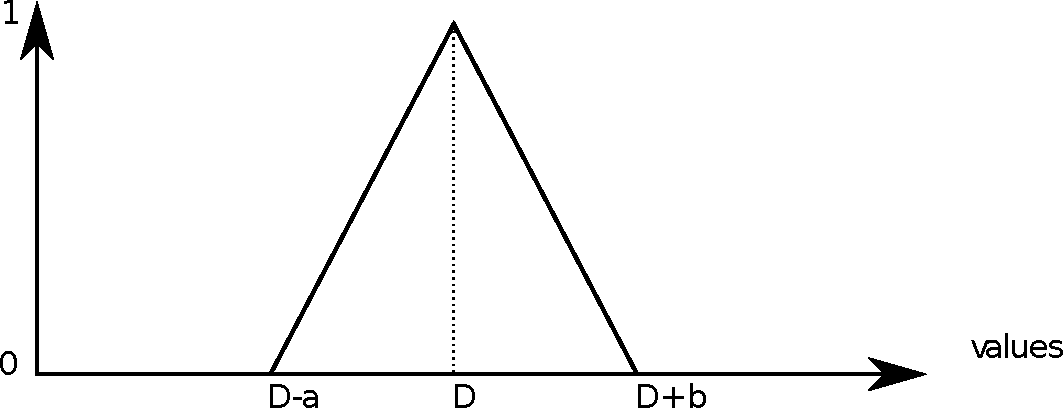
\includegraphics[scale=0.25]{./graphs/triangular.pdf}

}
\end{center}
%\centerline{ 
\psfig{file=./graphs/Y-time-point.eps}}
\vspace*{10pt}
\fcaption{\label{fig:triangular-dist}Example of fuzzy number.}
%  \label{fig:fuzzy-validity-period}
\vspace*{13pt}

If this modal value $m$ is unique, then $M$ is referred to as a \emph{fuzzy number}. 
%In other words, if the core of a fuzzy interval is a singleton, it is referred to as a fuzzy number (Figure \ref{fig:triangular-dist}).

A simple form of the membership function of a fuzzy interval is a trapezoidal function (Figure \ref{fig:trapezoidal-dist}). It can be shown that such a membership function $\mu_T$ for a fuzzy interval $T$ is convex and normalized. Four real values, denoted $\alpha$, $\beta$, $\gamma$ and $\delta$ suffice to represent a trapezoidal membership function of a fuzzy interval. In this work, a fuzzy interval defined as such will be noted as $\left[\alpha, \beta, \gamma, \delta\right]$. The corresponding membership function definition for this $\mu_T$ is then given by:

\begin{align}
\mu_T : & \quad \mathbb{R} \rightarrow \left[0,1\right] \\
 : & \quad x \rightarrow
\begin{cases}
1 & \mbox{ if } x \in [\beta,\gamma] \\
0 & \mbox{ if } x > \delta \vee x < \alpha \\
\frac{x-\alpha}{\beta - \alpha} & \mbox{ if } x \in [\alpha,\beta[ \\
\frac{\delta -x}{\delta - \gamma} & \mbox{ if } x \in ]\gamma,\delta] \\
\end{cases}
\end{align}


\vspace*{13pt}
\begin{center}
{
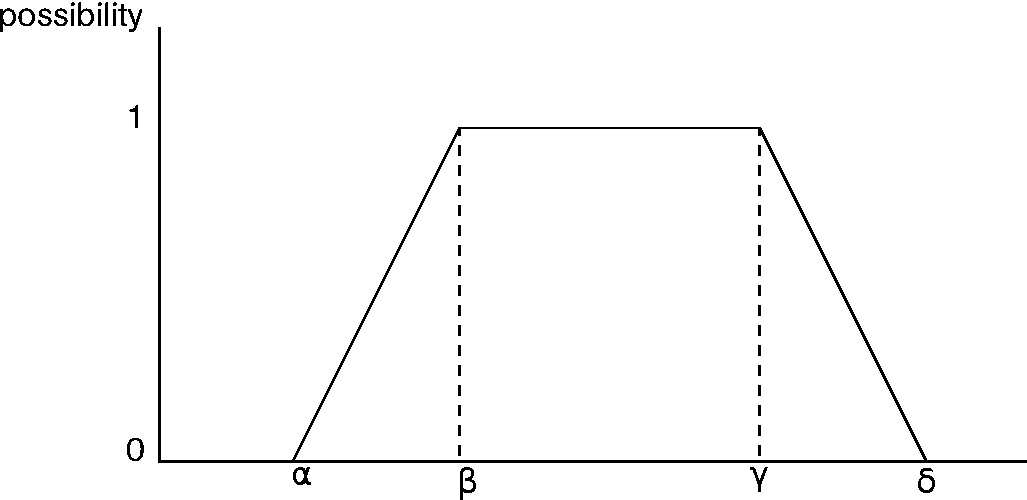
\includegraphics[scale=0.25]{./graphs/trapezoidalDistribution.pdf}

}
\end{center}
%\centerline{ 
\psfig{file=./graphs/Y-time-point.eps}}
\vspace*{10pt}
\fcaption{\label{fig:trapezoidal-dist}Example of fuzzy interval.}
%  \label{fig:fuzzy-validity-period}
\vspace*{13pt}
%\def\JPicScale{0.5}
%\begin{figure}[h!]
%  \centering
%  %%Created by jPicEdt 1.4.1_03: mixed JPIC-XML/LaTeX format
%%Thu Nov 17 17:57:10 CET 2011
%%Begin JPIC-XML
%<?xml version="1.0" standalone="yes"?>
%<jpic x-min="5" x-max="125" y-min="5" y-max="75" auto-bounding="true">
%<multicurve fill-style= "none"
%	 points= "(10,10);(10,10);(10,60);(10,60)"
%	 right-arrow= "head"
%	 />
%<multicurve fill-style= "none"
%	 points= "(10,10);(10,10);(110,10);(110,10)"
%	 right-arrow= "head"
%	 />
%<multicurve fill-style= "none"
%	 points= "(30,10);(30,10);(50,60);(50,60)"
%	 />
%<multicurve fill-style= "none"
%	 stroke-color= "#ccccff"
%	 points= "(70,60);(70,60);(90,10);(90,10)"
%	 />
%<text fill-style= "none"
%	 stroke-color= "#ff0033"
%	 stroke-width= "0.95"
%	 text-vert-align= "center-v"
%	 anchor-point= "(125,40)"
%	 text-frame= "noframe"
%	 text-hor-align= "center-h"
%	 >
%
%</text>
%<text fill-style= "none"
%	 stroke-color= "#ff0033"
%	 stroke-width= "0.95"
%	 text-vert-align= "center-v"
%	 anchor-point= "(30,5)"
%	 text-frame= "noframe"
%	 text-hor-align= "center-h"
%	 >
%$\alpha$
%</text>
%<text fill-style= "none"
%	 stroke-color= "#ff0033"
%	 stroke-width= "0.95"
%	 text-vert-align= "center-v"
%	 anchor-point= "(50,5)"
%	 text-frame= "noframe"
%	 text-hor-align= "center-h"
%	 >
%$\beta$
%</text>
%<text fill-style= "none"
%	 stroke-color= "#ff0033"
%	 stroke-width= "0.95"
%	 text-vert-align= "center-v"
%	 anchor-point= "(90,5)"
%	 text-frame= "noframe"
%	 text-hor-align= "center-h"
%	 >
%$\delta$
%</text>
%<text fill-style= "none"
%	 stroke-color= "#ff0033"
%	 stroke-width= "0.95"
%	 text-vert-align= "center-v"
%	 anchor-point= "(5,60)"
%	 text-frame= "noframe"
%	 text-hor-align= "center-h"
%	 >
%1
%</text>
%<text fill-style= "none"
%	 stroke-color= "#ff0033"
%	 stroke-width= "0.95"
%	 text-vert-align= "top"
%	 anchor-point= "(110,75)"
%	 text-rotation= "90"
%	 text-frame= "noframe"
%	 text-hor-align= "center-h"
%	 stroke-style= "dotted"
%	 >
%
%</text>
%<text fill-style= "none"
%	 text-vert-align= "center-v"
%	 anchor-point= "(45,70)"
%	 text-frame= "noframe"
%	 text-hor-align= "center-h"
%	 >
%
%</text>
%<text fill-style= "none"
%	 stroke-color= "#ff0033"
%	 stroke-width= "0.95"
%	 text-vert-align= "center-v"
%	 anchor-point= "(5,5)"
%	 text-frame= "noframe"
%	 text-hor-align= "center-h"
%	 >
%0
%</text>
%<text fill-style= "none"
%	 text-vert-align= "center-v"
%	 anchor-point= "(15,65)"
%	 text-frame= "noframe"
%	 text-hor-align= "center-h"
%	 >
%membership degree
%</text>
%<multicurve fill-style= "none"
%	 points= "(50,60);(50,60);(70,60);(70,60)"
%	 />
%<multicurve fill-style= "none"
%	 polydots-size-linewidth-scale= "2.5"
%	 polydots-style= "polydots-circle"
%	 stroke-color= "#3300cc"
%	 polydots-scale-v= "1"
%	 polydots-angle= "0"
%	 polydots-scale-h= "1"
%	 stroke-dasharray= "1;1"
%	 polydots-superimpose= "false"
%	 points= "(50,60);(50,60);(50,10);(50,10)"
%	 polydots-size-minimum= "0.7"
%	 stroke-style= "dashed"
%	 />
%<multicurve fill-style= "none"
%	 stroke-dasharray= "1;1"
%	 points= "(70,60);(70,60);(70,10);(70,10)"
%	 stroke-style= "dashed"
%	 />
%<text fill-style= "none"
%	 stroke-color= "#ff0033"
%	 stroke-width= "0.95"
%	 text-vert-align= "center-v"
%	 anchor-point= "(70,5)"
%	 text-frame= "noframe"
%	 text-hor-align= "center-h"
%	 >
%$\gamma$
%</text>
%</jpic>
%%End JPIC-XML
%LaTeX-picture environment using emulated lines and arcs
%You can rescale the whole picture (to 80% for instance) by using the command \def\JPicScale{0.8}
\ifx\JPicScale\undefined\def\JPicScale{1}\fi
\unitlength \JPicScale mm
\begin{picture}(125,75)(0,0)
\linethickness{0.3mm}
\put(10,10){\line(0,1){50}}
\put(10,60){\vector(0,1){0.12}}
\linethickness{0.3mm}
\put(10,10){\line(1,0){100}}
\put(110,10){\vector(1,0){0.12}}
\linethickness{0.3mm}
\multiput(30,10)(0.12,0.3){167}{\line(0,1){0.3}}
\linethickness{0.3mm}
\multiput(70,60)(0.12,-0.3){167}{\line(0,-1){0.3}}
\put(125,40){\makebox(0,0)[cc]{}}

\put(30,5){\makebox(0,0)[cc]{$\alpha$}}

\put(50,5){\makebox(0,0)[cc]{$\beta$}}

\put(90,5){\makebox(0,0)[cc]{$\delta$}}

\put(5,60){\makebox(0,0)[cc]{1}}

\put(110,75){\makebox(0,0)[tc]{}}

\put(45,70){\makebox(0,0)[cc]{}}

\put(5,5){\makebox(0,0)[cc]{0}}

\put(15,65){\makebox(0,0)[cc]{membership degree}}

\linethickness{0.3mm}
\put(50,60){\line(1,0){20}}
\linethickness{0.3mm}
\multiput(50,10)(0,1.96){26}{\line(0,1){0.98}}
\linethickness{0.3mm}
\multiput(70,10)(0,1.96){26}{\line(0,1){0.98}}
\put(70,5){\makebox(0,0)[cc]{$\gamma$}}

\end{picture}

%  \caption{Trapezoidal membership function}
%  \label{fig:trapezoidal}
%\end{figure}

The most convenient form of the membership function of a fuzzy number is a triangular form. It can be shown that such a membership function $\mu_M$ for a fuzzy number $M$ is convex and normalized. Three real values, denoted by $a$, $b$ and $D$, suffice to represent a triangular membership function of a fuzzy number and in this work, a fuzzy number defined as such will be noted as $\left[D, a, b \right]$. Here:
\begin{itemize}
\item
$D$ denotes the single value in the core of $M$
\item
$D-a$ is then $\inf \{u \in \mathbb{R} : \mu_{M}(u) > 0\}$
\item
$D+b$ is then $\sup \{u \in \mathbb{R} : \mu_{M}(u) > 0\}$
\end{itemize}

The membership function of such a fuzzy number is then given by:

\vspace{-10pt}

\begin{align}
\mu_M :   \mathbb{R} \rightarrow \left[0,1\right] :  x \rightarrow \nonumber\\
\begin{cases}
\nonumber
0 & \mbox{ if } \left(x < D-a\right) \vee \left(x > D+b\right) \\
\frac{\left[x-\left(D-a\right)\right]}{a} & \mbox{ if } \left(x \geq D-a\right) \wedge (x \leq D)  \\
-\frac{\left[x-\left(D+b\right)\right]}{b} & \mbox{ if } \left(x \geq D\right) \wedge (x \leq D+b)
\end{cases}
\end{align}

%\begin{figure}[h!]
%  \centering
%  %%Created by jPicEdt 1.4.1_03: mixed JPIC-XML/LaTeX format
%%Thu Jan 12 17:26:56 CET 2012
%%Begin JPIC-XML
%<?xml version="1.0" standalone="yes"?>
%<jpic x-min="-2.5" x-max="60" y-min="-2" y-max="32.5" auto-bounding="true">
%<multicurve right-arrow= "head"
%	 fill-style= "none"
%	 points= "(0,0);(0,0);(55,0);(55,0)"
%	 />
%<multicurve right-arrow= "head"
%	 fill-style= "none"
%	 points= "(0,0);(0,0);(0,30);(0,30)"
%	 />
%<text right-arrow= "head"
%	 fill-style= "none"
%	 text-vert-align= "center-v"
%	 anchor-point= "(-2.5,27.5)"
%	 text-frame= "noframe"
%	 text-hor-align= "center-h"
%	 >
%1
%</text>
%<text right-arrow= "head"
%	 fill-style= "none"
%	 text-vert-align= "center-v"
%	 anchor-point= "(-2.5,0)"
%	 text-frame= "noframe"
%	 text-hor-align= "center-h"
%	 >
%0
%</text>
%<text right-arrow= "head"
%	 fill-style= "none"
%	 text-vert-align= "center-v"
%	 anchor-point= "(15,32.5)"
%	 text-rotation= "135"
%	 text-frame= "noframe"
%	 text-hor-align= "center-h"
%	 >
%Membership Degree
%</text>
%<multicurve fill-style= "none"
%	 points= "(4,0);(4,0);(15,27.5);(15,27.5)"
%	 />
%<multicurve fill-style= "none"
%	 points= "(15,27.5);(15,27.5);(42,0);(42,0)"
%	 />
%<text fill-style= "none"
%	 text-vert-align= "center-v"
%	 anchor-point= "(60,0)"
%	 text-frame= "noframe"
%	 text-hor-align= "center-h"
%	 >
%Time
%</text>
%<text fill-style= "none"
%	 text-vert-align= "center-v"
%	 anchor-point= "(16,-2)"
%	 text-frame= "noframe"
%	 text-hor-align= "center-h"
%	 >
%$D$
%</text>
%<text fill-style= "none"
%	 text-vert-align= "center-v"
%	 anchor-point= "(4,-2)"
%	 text-frame= "noframe"
%	 text-hor-align= "center-h"
%	 >
%$D-a$
%</text>
%<text fill-style= "none"
%	 text-vert-align= "center-v"
%	 anchor-point= "(42,-2)"
%	 text-frame= "noframe"
%	 text-hor-align= "center-h"
%	 >
%$D+b$
%</text>
%</jpic>
%%End JPIC-XML
%LaTeX-picture environment using emulated lines and arcs
%You can rescale the whole picture (to 80% for instance) by using the command \def\JPicScale{0.8}
\ifx\JPicScale\undefined\def\JPicScale{1}\fi
\unitlength \JPicScale mm
\begin{picture}(60,32.5)(0,0)
\linethickness{0.3mm}
\put(0,0){\line(1,0){55}}
\put(55,0){\vector(1,0){0.12}}
\linethickness{0.3mm}
\put(0,0){\line(0,1){30}}
\put(0,30){\vector(0,1){0.12}}
\put(-2.5,27.5){\makebox(0,0)[cc]{1}}

\put(-2.5,0){\makebox(0,0)[cc]{0}}

\put(15,32.5){\makebox(0,0)[cc]{Membership Degree}}

\linethickness{0.3mm}
\multiput(4,0)(0.12,0.3){92}{\line(0,1){0.3}}
\linethickness{0.3mm}
\multiput(15,27.5)(0.12,-0.12){225}{\line(0,-1){0.12}}
\put(60,0){\makebox(0,0)[cc]{Time}}

\put(16,-2){\makebox(0,0)[cc]{$D$}}

\put(4,-2){\makebox(0,0)[cc]{$D-a$}}

\put(42,-2){\makebox(0,0)[cc]{$D+b$}}

\end{picture}

%  \caption{Triangular membership function.}
%  \label{fig:triangular}
%\end{figure}



\subsection{\label{subsec:interval-evaluation-by-ill-known-constraints}Interval Evaluation by Ill-known Constraints}
The problem of interval evaluation is more generally explained in \cite{Pons2011}: the need exists to know if all points in a crisp interval $I$ reside between the boundaries of an ill-known interval $\left[ X , Y \right]$. In \cite{Pons2011}, the notion of an \emph{ill-known constraint} is introduced:

\begin{definition}
Given a universe $U$, an ill-known constraint $C$ on a set $A \subseteq U$ is specified by means of a binary relation $R \subseteq U^{2}$ and a fixed, ill-known value denoted by its possibilistic variable $V$ over $U$, i.e.:
\begin{align}
\label{eq:ill-known-constraint}
C \triangleq (R,V)
\end{align}
Set $A$ now satisfies the constraint if and only if:
\begin{align}
\forall a \in A : (a,V) \in R
\end{align}
\end{definition}

An example of an ill-known constraint is $C_{ex} \triangleq (<, X)$. Some set $A$ then satisfies $C_{ex}$ if $\forall a \in A : a < X$, given possibilistic variable $X$.

The satisfaction of a constraint $C \triangleq (R,V)$ by a set $A$ is basically still a Boolean matter, but due to the uncertainty about the ill-known value $V$, it can be uncertain whether $C$ is satisfied by $A$ or not \cite{Pons2011}. In fact, this satisfaction now behaves as a proposition. Based on the possibility distribution $\pi_{V}$ of $V$, the possibility and necessity that $A$ satisfies $C$ can be found. This proposition can thus be seen as a possibilistic variable on $\mathbb{B}$. The required possibility and necessity are:

\vspace{-10pt}

\begin{align}
\Pos(A\text{ satisfies }C) & =\\
\nonumber
\min_{a \in A}\left(\sup_{(a,w) \in R}\pi_{V}(w)\right) \label{ill-known-pos}\\
\Nec(A\text{ satisfies }C) & =\\
\nonumber
\min_{a \in A}\left(\inf_{(a,w) \notin R} 1-\pi_{V}(w)\right) \label{ill-known-nec}
\end{align}

So far, we have shown how it can be verified if a set satisfies or not an ill-known constraint.

\begin{example}

\vspace*{13pt}
\begin{center}
{
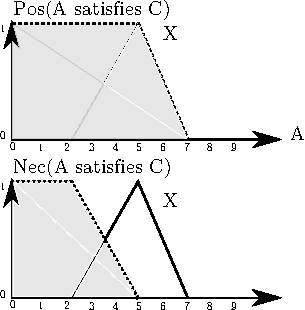
\includegraphics[scale=1]{./graphs/example-ill-known.pdf}
}
\end{center}
%\centerline{ 
\psfig{file=./graphs/Y-time-point.eps}}
\vspace*{10pt}
\fcaption{\label{fig:example-ill-known}Example of the evaluation of the ill-known constraint $C \triangleq (\leq, X)$. Possibility and necessity measures are shown in grey the upper and lower graphics respectively. }
%  \label{fig:fuzzy-validity-period}
\vspace*{13pt}


 Consider an ill-known value given by $X = \left[5, 3, 2 \right]$. $C \triangleq (\leq, X)$ is the ill-known constraint. The set $A$ is $A \subseteq \R^+$. Then, the evaluation of the possibility and the neccesity are obtained from \eqref{ill-known-pos} and \eqref{ill-known-nec} respectively. (See Figure \ref{fig:example-ill-known}).
 
\begin{align}
\Pos(A\text{ satisfies }C) & =\\
\nonumber
\min_{a \in A}\left(\sup_{a \leq R}\pi_{X}(w)\right)\\
\Nec(A\text{ satisfies }C) & =\\
\nonumber
\min_{a \in A}\left(\inf_{a > w} 1-\pi_{X}(w)\right) 
\end{align}




\end{example}





 However, from the examples at the beginning of this section, it is observed that Boolean combinations of constraints are required. For example, the problem of interval evaluation as explained earlier requires that all elements of an interval $[a,b]$ are larger than a value $X$ and at the same time smaller than a value $Y$, which implies that a conjunctive Boolean combination of both constraints must be satisfied. To allow Boolean combinations of constraints, the following definitions are introduced.
\begin{definition}
\label{def:set-evaluation}
Consider a universe $U$, an $n$-ary vector $\mathbf{C}$ of constraints and a Boolean function $\bool:\mathbb{B}^{n}\rightarrow\mathbb{B}$. An evaluation function is defined by:
\begin{equation}
\lambda:\Pow(U)\rightarrow\mathbb{B}:A\mapsto\bool\Big(C_{1}(A),...,C_{n}(A)\Big).
\end{equation}
\end{definition}
Definition \ref{def:set-evaluation} presents the definition of an evaluation function that evaluates a Boolean combination of some basic constraints. Informally, it states that a set $A$ passes the evaluation made by $\lambda$ if the Boolean combination of some propositions equals $T$. This crisp definition can be generalized to the case of ill-known constraints.
\begin{definition}
\label{def:ill-known-sets}
Consider a universe $U$, an $n$-ary vector $\mathbf{C}$ of ill-known constraints and a Boolean function $\bool:\mathbb{B}^{n}\rightarrow\mathbb{B}$. The uncertainty about the evaluation of a set $A$ by an evaluation function $\lambda$ is then given by:
\begin{equation}
\forall A\in\Pow(U):\pi_{\lambda(A)}=\widetilde{\bool}\Big(\pi_{C_1(A)},...,\pi_{C_n(A)}\Big)\\
\end{equation}
Hereby, $\widetilde{\bool}$ is the possibilistic extension of $\bool$.
\end{definition}
It is well known that any Boolean function $\bool$ can be cast to a canonical form~\cite{McCluskey1965}, requiring only the logical conjunction $\wedge$, logical disjunction $\vee$ and logical negation. Therefore, only the case of Boolean conjunction, Boolean disjunction and Boolean negation will be treated within the scope of this paper. By applying the possibilistic extensions of $\wedge$, $\vee$ and $\neg$, concrete equations are obtained for the calculations of uncertainty about the evaluation of a set by means of an evaluation function $\lambda$. In the case of conjunction (i.e., $\bool=\wedge$), the inference of uncertainty about the evaluation of a set reduces to:
\begin{eqnarray}
\label{eq:conjunctive1}
\forall A\in\Pow(U):\Pos(\lambda(A))&=\\
\nonumber
\min_{i=1}^n\Pos\left(C_i(A)\right)\\
\label{eq:conjunctive2}
\forall A\in\Pow(U):\Nec(\lambda(A))&=\\
\nonumber
\min_{i=1}^n\Nec\left(C_i(A)\right).
\end{eqnarray}
In the case of disjunction (i.e. $\bool=\vee$), the inference of uncertainty about the evaluation of a set reduces to:
\begin{eqnarray}
\label{eq:disjunctive}
\forall A\in\Pow(U):\Pos(\lambda(A))&=\\
\nonumber
\max_{i=1}^n\Pos\left(C_i(A)\right)\\
\forall A\in\Pow(U):\Nec(\lambda(A))&=\\
\nonumber
\max_{i=1}^n\Nec\left(C_i(A)\right).
\end{eqnarray}
Note that by using the functions $\min$ and $\max$ here, there is an implicit assumption that the possibilistic variables $\pi_{C_i}$ are mutual $\min$-dependent in the sense of De Cooman (i.e. non-interactive). For an extensive reading on (in)dependency of possibilistic variables, the reader is referred to~\cite{GertDeCooman1997b},\cite{GertDeCooman1997a},\cite{GertDeCooman1997}. In case of $\neg$, we get:
\begin{eqnarray}
\label{eq:negation}
\forall A\in\Pow(U):\Pos(\neg\lambda(A))&=\\
\nonumber
1-\Nec(\lambda(A))\\
\forall A\in\Pow(U):\Nec(\neg\lambda(A))&=\\
\nonumber
1-\Pos(\lambda(A)).
\end{eqnarray}

\begin{example}
Consider that we want to check if crisp interval $I = \left[j, k\right]$ is included in $\left[X, Y\right]$, 2 ill-known constraints are constructed:

%We assume that $X$ specifies the lower bound and $Y$ the upper bound for a given interval, we want to known whether all points in the interval are larger than or equal to $X$ and smaller than or equal to $Y$. Therefore, we consider two ill-known constraints:

\vspace{-10pt}

\begin{eqnarray}
C_1 & \triangleq\left(\geq,X\right)\\
C_2 & \triangleq\left(\leq,Y\right)
\end{eqnarray}

To calculate the possibility and necessity concerning a conjunction of constraints, the $\min$ operator can be used. The possibility and necessity of $I$ being included in $\left[X, Y\right]$ are now: %satisfying both constraints is then:

\vspace{-10pt}

\begin{align}
\label{eq:interval-pos}
\Pos(I\text{ satisfies }C_1\ and\ C_2) & =\\
\nonumber
\min_{a \in I}\left(\sup_{a \geq w}\pi_{X}(w),\sup_{a \leq v}\pi_{Y}(v)\right)\\
\label{eq:interval-nec}
\Nec(I\text{ satisfies }C_1\ and\ C_2) & =\\
\nonumber
\min_{a \in I}\left(\inf_{a < w} 1-\pi_{X}(w),\inf_{a > v} 1-\pi_{Y}(v)\right).
\end{align}
\end{example}

There is a special boolean combination of constraints that is of particular interest:
\begin{definition}
\emph{Convex combination of ill-known constraints}. Consider the $C_1$ and $C_2$ two ill-known constraints. A convex combination of the constraints is given by:
\begin{align}
\label{eq:convex-combination}
CC \triangleq \left \lbrace C_1 \wedge C_2 \right \rbrace
\end{align}
In a more general way, it is possible to define the convex combination of an n-ary vector  $\mathbf{C}$ of constraints:
\begin{align}
\label{eq:nary-convex-combination}
CC \triangleq \left \lbrace C_1 \wedge \ldots \wedge C_n \right \rbrace
\end{align}
\end{definition}

\begin{theorem}
\label{th:convex-combination-ill-known-constraints}
Consider the convex combination $CC$ of any n-ary vector $\mathbf{C} = \left \lbrace C_{1_{Z_1}}, \ldots, C_{n_{Z_n}} \right \rbrace$ of constraints over the ill-known variables $Z_1, \ldots, Z_n$. Then, if $\pi_{C_1(Z_1)}, \ldots, \pi_{C_n(Z_n)}$ are convex, then  $\pi_{CC}$ is also convex.
\end{theorem}

\begin{proof}
Let $CC \triangleq \left \lbrace C_{1_{Z_1}}, \ldots, C_{n_{Z_n}}  \right \rbrace$. Then:
\begin{align}
\label{eq:proof-convex1}
\pi_{CC} \left( \lambda x_1 + \left( 1 - \lambda \right)x_2 \right) = \\
\min  \big( \pi_{C_1(Z_1)}\left( \lambda x_1 + \left( 1 - \lambda \right)x_2 \right), \ldots,\\
   \pi_{C_n(Z_n)}\left( \lambda x_1 + \left( 1 - \lambda \right)x_2 \right)  \big)
\end{align}
Since $\pi_{C_1(Z_1)}, \ldots, \pi_{C_n(Z_n)}$ are convex:
\begin{align}
\label{eq:proof-convex2}
\pi_{C_1(Z_1)} \left(\lambda x_1 + \left( 1 - \lambda \right)x_2  \right) \geqq \\
\nonumber
\min \big(\pi_{C_1(Z_1)} \left( x_1 \right),\pi_{C_1(Z_1)} \left( x_2 \right)  \big)\\
\nonumber
\vdots \\
\nonumber
\pi_{C_n(Z_n)} \left(\lambda x_1 + \left( 1 - \lambda \right)x_2  \right) \geqq \\
\nonumber
\min \big(\pi_{C_n(Z_n)} \left( x_1 \right),\pi_{C_n(Z_n)} \left( x_2 \right) \big) 
\end{align}
Then, by using equation \eqref{eq:proof-convex1}:
\begin{align}
\label{eq:proof-convex3}
\pi_{CC} \left( \lambda x_1 + \left( 1 - \lambda \right)x_2 \right) \geqq  \\
\nonumber
\min \big( \min \left(\pi_{C_1(Z_1)} \left( x_1 \right),\pi_{C_1(Z_1)} \left( x_2 \right) \right),\\
\nonumber
\ldots, \min \left(\pi_{C_n(Z_n)} \left( x_1 \right),\pi_{C_n(Z_n)} \left( x_2 \right) \right) \big)
\end{align}
Which is equivalent to the following:
\begin{align}
\label{eq:proof-convex4}
\pi_{CC} \left( \lambda x_1 + \left( 1 - \lambda \right)x_2 \right) \geqq  \\
\nonumber
\min \big( \min \left(\pi_{C_1(Z_1)} \left( x_1 \right), \ldots, \pi_{C_n(Z_n)} \left( x_1 \right) \right),\\
\nonumber
\ldots, \min \left(\pi_{C_1(Z_1)} \left( x_2 \right), \ldots, \pi_{C_n(Z_n)} \left( x_2 \right) \right) \big)
\end{align}
Finally we obtain:
\begin{align}
\label{eq:proof-convex5}
\pi_{CC} \left( \lambda x_1 + \left( 1 - \lambda \right)x_2 \right) \geqq  \\
\nonumber
\min \big(\pi_{CC} \left( x_1 \right), \pi_{CC} \left( x_2 \right) \big)
\end{align}
\end{proof}

Sometimes, an ill-known value might be specified by a convex combination of ill-known constraints. This allow to define ill-known values by means of relationships with respect to other ill-known points.

%\begin{definition}
%\emph{Ill-known point defined by ill-known constraints}
%Consider a universe $U$, an n-ary vector $\mathbf{C}$ of ill-known constraints and a Boolean function $\bool:\mathbb{B}^{n}\rightarrow\mathbb{B}$. An ill-known value $X$ is defined by:
%\begin{align}
%\label{eq:ill-known-value-def-by-const}
%X \in \Pow(U):\pi_{X}=\widetilde{\bool}\Big(\pi_{C_1(Z_1)},...,\pi_{C_n(Z_n)}\Big)\\
%\end{align} 
%\end{definition}

\begin{definition}
\label{def:convex-combination-ill-known-constraints}
Consider a universe $U$, $X$ an ill-known value and $CC \triangleq \left \lbrace C_{1_{Z_1}}, \ldots, C_{n_{Z_n}}  \right \rbrace$ a convex combination of ill-known constraints over the variables $Z_1, \ldots, Z_n$. The value $X$ is defined by means of the convex combination:
\begin{align}
\label{eq:ill-known-value-by-convex-constraints}
X \triangleq CC 
\end{align}

The uncertainty about the evaluation of an ill-known value $X$ is given by:
\begin{align}
\label{eq:ill-known-value-def-by-const-unc}
X \in \Pow(U):\pi_{X}=\pi_{CC}
\end{align} 
Note that $\pi_{X}$ is convex since $\pi_{CC}$ is convex as demonstrated in theorem \ref{th:convex-combination-ill-known-constraints}.
\end{definition}


\begin{example}
Consider the ill-known values $X = \left[12, 2, 2\right]$ and $Y = \left[18, 2, 1 \right]$. The ill-known value $Z$ is defined using the convex combination $CC$ of constraints $C_1$ and $C_2$:
\begin{align}
\nonumber
CC \triangleq \left \lbrace C_1\left(>,X\right) \wedge C_2(\leq,Y) \right \rbrace \\
\nonumber
Z \triangleq CC
\end{align}
$Z$ is a fuzzy interval defined by a trapezoidal shape given by $\left[12,\ 14,\ 18,\ 19 \right]$.
Figure \ref{fig:example-ill-known-by-const} illustrates the relations among the variables $X$, $Y$ and $Z$.
\end{example}

\vspace*{13pt}
\begin{center}
{
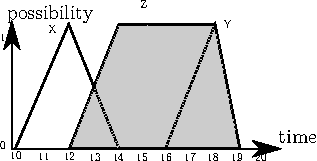
\includegraphics[scale=1]{./graphs/ill-known-by-constraints.pdf}

}
\end{center}
%\centerline{ 
\psfig{file=./graphs/Y-time-point.eps}}
\vspace*{10pt}
\fcaption{\label{fig:example-ill-known-by-const}Ill-known values $X$ and $Y$. The grey area represents the ill-known value $Z$ defined by the convex combination of the two ill-known constraints $C_1$ and $C_2$.}
\vspace*{13pt}

%\paragraph{Example} Consider the ill-known values $X = \left[5, 2, 8\right]$ and $Y = \left[9, 7, 10 \right]$. The knowledge about the evaluation of the interval $\left[a, b \right]$  is given by the expressions \eqref{eq:interval-pos},\eqref{eq:interval-nec}.  Figure~\ref{fig:3d-possibility} shows a 3D plot of the possibility that an interval $[a,b]$ passes the evaluations specified by the ill-known constraints. Note the triangular form for the resulting possibility distribution since the condition $a \leq b$ holds.
%
%\begin{figure}[h!]
%\centering
%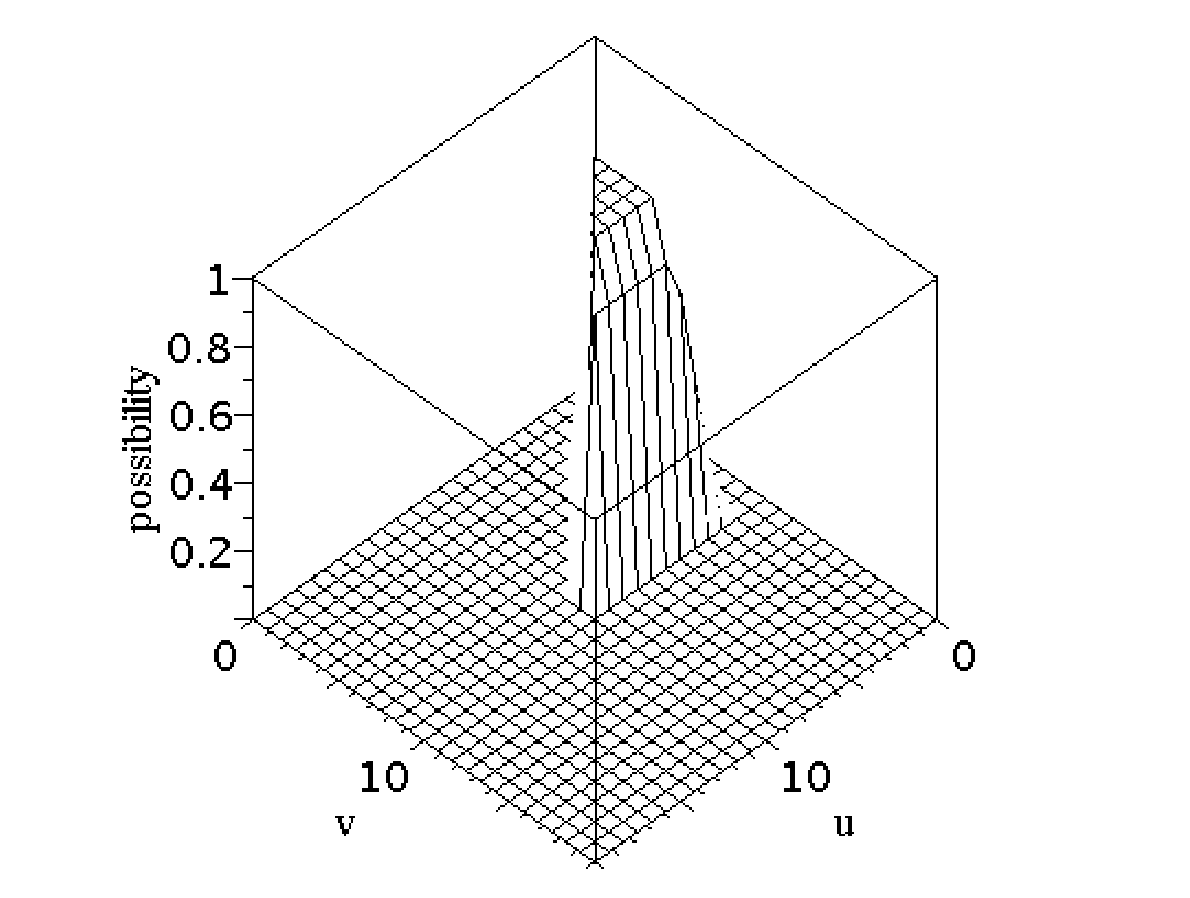
\includegraphics[scale=0.4]{graphs/3D_possibility.eps}
%\caption{Possibility of evaluation for the interval $[a,b]$.}
%\label{fig:3d-possibility}
%\end{figure}
%The necessity plot is obtained in a similar way and is shown in Figure~\ref{fig:3d-necessity}. Notice that the necessity measure is not normalized because the supports of $X$ and $Y$ overlap.
%\begin{figure}[h!]
%\centering
%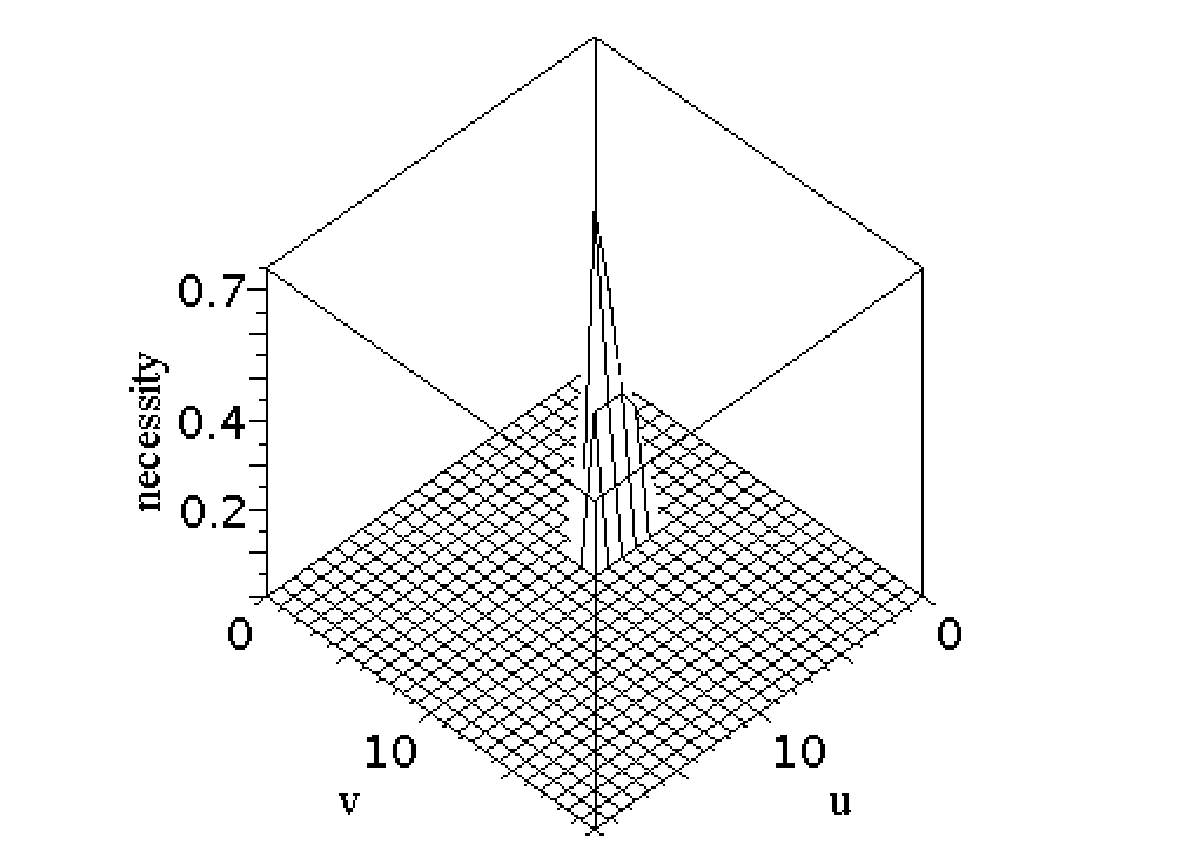
\includegraphics[scale=0.4]{graphs/3D_necessity.eps}
%\caption{Necessity of evaluation for the interval $[a,b]$.}
%\label{fig:3d-necessity}
%\end{figure}





%%Imperfection and time: modelling imperfect time (generally)


%Modelling imperfect time in temporal databases


%Guy's suggestion: instead of imprecision, use imperfection which is more general.
\subsubsection{Imperfection and time}
Representing imprecision and its semantics when dealing with time has been studied for a long time. Several proposals for representing and computing imprecise time indications can be found in \cite{DeCaluwe1997,DeTre1997}. Also, the changes between several granularities can be seen as a source of imprecision \cite{Devos1998}.

In the proposal section we will consider two kinds of imperfection:
\begin{itemize}
\item \textbf{Imperfection in the database} the knowledge about the temporal data contains some imperfection. E.g., a database record shows that \emph{`The car is in the garage around April.'}
 \item \textbf{Imprecision in the query specification} denotes the imprecision in the specification of temporal criteria by the user, when querying. E.g., \emph{`The user wants to obtain a car which is red and which is in the garage around April.'}
\end{itemize}

\subsubsection{Representation}
Several proposals for managing uncertain time in a database exist. Some proposals work with rough sets \cite{Qiang2009}, other proposals rely on possibility distributions for representing uncertainty in time \cite{Dyreson1998,Garrido2009,Galindo2001}. In order to compare temporal possibility distributions, extensions of the classical Allen's operators \cite{Allen1983} are defined in \cite{Ohlbach2004,Nagypal2003,Dubois2003a,Schockaert2008}.
%In the proposal section, we will follow the representation by means of possibility distributions, in order to work with both satisfaction and dissatisfaction degrees. Also, in order to work properly with fuzzy operators, the underlying domain should be numeric. 
% Take a look into this:
%In this paper, the representation for the dates will follow the Julian Day Number (JDN) representation \cite{Dir96}.

%If the starting points and/or the end points of the interval representing the time are not known precisely, it is easy to fuzzify them, using, e.g., two triangular possibility distributions.


In order to deal with uncertainty in time intervals, several proposals are made. Here, two approaches are introduced: the first one, based on \emph{Fuzzy Validity Period}~\cite{Garrido2009} and the second one based on \emph{Possibilistic Valid-time Period}~\cite{JoseEnriquePons2012}.

\begin{definition}
A \textbf{Fuzzy Validity Period} (\emph{FVP}) is defined as a fuzzy time interval specifying when the data regarding an object is valid. A fuzzy time interval is then the fuzzification of a crisp time interval.
\end{definition}
Several options to transform possibility distributions corresponding to the fuzzy starting point and the fuzzy end point into one consistent FVP exist \cite{Garrido2009}, e.g (Fig. \ref{fig:fuzzy-validity-period}):
\begin{itemize}
\item The \textbf{convex hull} approach is the most intuitive approach. The resulting FVP is the convex hull of the union of both fuzzy sets.
\item The \textbf{uncertainty preserving} approach is less intuitive but more realistic. The amount of uncertainty is maintained at the edges of the possibility distribution representing the FVP \cite{Garrido2009}.
\end{itemize}

%%%%%%
% FUZZY VALIDITY PERIOD
%%%%%%
\vspace*{13pt}
\begin{center}
{
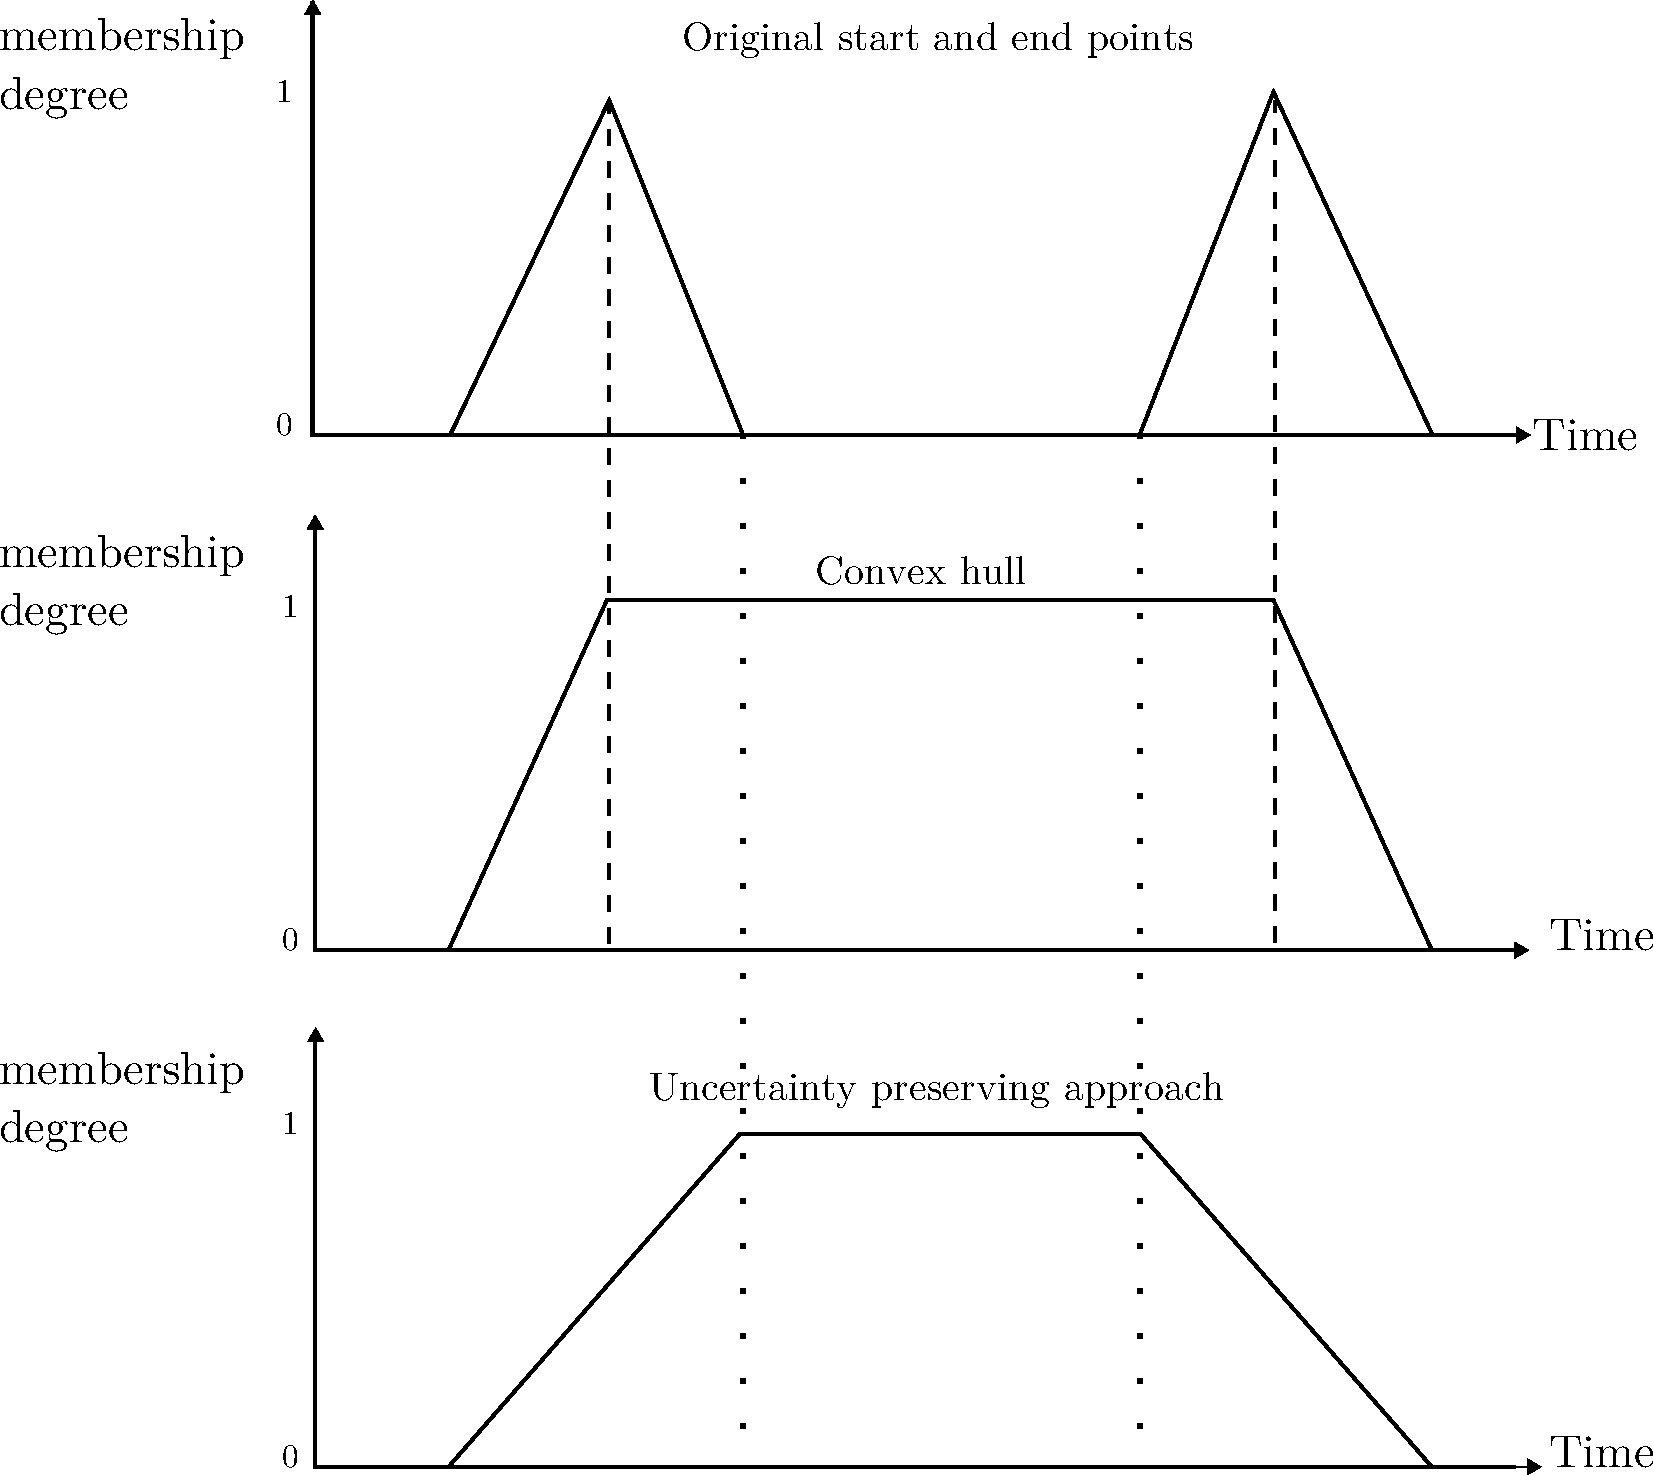
\includegraphics[scale=0.25]{./graphs/comparisoncv.pdf}

}
\end{center}
%\centerline{ 
\psfig{file=./graphs/Y-time-point.eps}}
\vspace*{10pt}
\fcaption{\label{fig:fuzzy-validity-period}Transformation to obtain the FVP. The top graph shows the two triangular possibility distributions. The middle graph shows the convex hull validity period, the bottom one shows the result of the second transformation, which maintains the imprecision.}
%  \label{fig:fuzzy-validity-period}
\vspace*{13pt}

\begin{definition}
A \textbf{Possibilistic Valid-time Period} (\emph{PVP}) is an ill-known interval in time specifying when the data regarding an object is valid.
\end{definition}
A PVP is an ill-known interval in the sense of definition \ref{def;possibilistic-variable}, section \ref{subsec:possibilistic-variables}. Note that this representation is \emph{disjunctive}: the PVP represents only one crisp time interval, but that for some reason it is (partially) unknown.

The ill-known interval approach has many advantages from the representation by the FVP as demonstrated in \cite{Pons2011},\cite{Pons2012}. Table \ref{tbl:comparative-pvp-fvp} is a comparative between PVP and FVP. The following list defines the items in the comparative:

\begin{enumerate}
\item Domain: The domain of the possibility distribution modelled by the approach.
\item Implementation of relationships: How to implement a relationship.
\item Allen's relations: Are the Allen's relations defined?
\item Storage: The way the data is stored in the database.
\item Possibility measures: Does the framework provides always a possibility measure for any relation between the temporal elements?
\item Necessity measures:  Does the framework provides always a necessity measure for any relation between the temporal elements?
\end{enumerate}


%%
%% comparison table between pvp and fvp.
%%
\vglue13pt
%\begin{table}[htbp]
\tcap{Comparative PVP vs FVP}
%\centerline{\small DATA TYPES}
\vglue-6pt
\centerline{\small\baselineskip=13pt
\begin{tabular}{c p{2cm} p{2cm}}\\
Item & PVP & FVP\\
\hline
(1) & $\Pow(\R)$ & $\R$ \\
(2) & Ill-known constraints. & Ad-hoc operators. \\
(3) & $\checkmark$ & - \\
(4) & Two distributions one for each endpoint. & Only one distribution. \\ 
(5) & $\checkmark$ & $\checkmark$ \\
(6) & $\checkmark$ & - \\
\hline\\
\end{tabular}
\label{tbl:comparative-pvp-fvp}
} 

In the rest of the paper we will work only with PVP to represent valid-time intervals.


%\section{\label{sec:example}Example}
%\input{./sources/example.tex}

\section{\label{sec:time-rep}Time Representation}
%%%%%%%%%%%%%%%%%%%%%%%%%%%%%%%%%%%%%%%%%%%%%%%%%%%%%%%%%%%%%%%
%
% Time representation
%
%%%%%%%%%%%%%%%%%%%%%%%%%%%%%%%%%%%%%%%%%%%%%%%%%%%%%%%%%%%%%%%%

This section is devoted to specify the representation of time within the framework of the possibility theory. First of all, the specification for a single ill-known temporal point shall be explained. Then, the formal specification and the related constraints are given for an ill-known valid-time interval.

\subsection{\label{subsec:ill-known-point-rep}Ill-known time point}
An ill-known time point $X$ is a precise time point that for some reason, it is not fully specified. Note that $X$ has only one possible value but that value is unspecified.

\begin{definition}
\label{def:ill-known-time-point}
\emph{Ill-known time point}\\
Consider a time domain $\T$, uncertainty about the values of the ill-known time point $X$ is given by the possibility distribution $\pi_X$:
\begin{equation}
\label{eq:ill-known-time-point}
\Pi(X) = \pi_X(t) \in \left[0,1\right] , t \in \T
\end{equation}
\end{definition}

\begin{definition}
\label{def:ill-known-domain}
\emph{Domain for an ill-known time point}\\
Consider $\Pow(\T)$ the set of all the possibility distributions over $\T$, and the three fuzzy constants \emph{UNKNOWN} $=\left\lbrace 1/t, t \in \T \right\rbrace$, \emph{UNDEFINED} $=\left\lbrace 0/t, t \in \T \right\rbrace$ and \emph{NULL} $=\lbrace 1/$ \emph{UNKNOWN}, $1/$ \emph{UNDEFINED} $\rbrace$. The domain for an ill-known time point $X$ is given by: 
\begin{align}
\label{eq:ill-known-domain}
\Dom (X) =  \lbrace \Pow(\T) & \cup \mbox{\emph{UNKNOWN}} \\
\nonumber
&\cup \mbox{\emph{UNDEFINED}} \\
\nonumber
&\cup \mbox{\emph{NULL}} \rbrace
%
\end{align}
\end{definition}

It is also possible to specify an ill-known time point by just a set of ill-known constraints plus 



\subsubsection{\label{subsubsec:ill-known-time-datatypes}Datatypes}
The datatypes for an ill-known time point $X$ are shown in Table \ref{tbl:time-point-types}.
\vglue13pt
%\begin{table}[htbp]
\tcap{Data types for a time point}
\centerline{\small DATA TYPES}
\vglue-6pt
\centerline{\small\baselineskip=13pt
\begin{tabular}{c p{2cm} p{2cm}}\\
\hline
1 & A single time point &  $1/x, x \in \T$\\
2 & A possibility distribution in the numeric domain & A fuzzy number or a fuzzy interval.\\
3 & An unknown value & \textbf{UNKNOWN}$= \lbrace1/t, t \in \T \rbrace$\\
4 & An undefined value & \textbf{UNDEFINED}$= \lbrace 0/t, t \in \T \rbrace$\\
5 & A null value & \textbf{NULL} $=\lbrace 1/$Unknown, 1/Undefined $\rbrace$\\
\hline\\
\end{tabular}
\label{tbl:time-point-types}
}

%Example of different uses of the ill-known time value.
\begin{example}
Consider a historical database with data from diplomatic documents. The following fields are stored: the digital identifier \emph{ID} which is the primary key  and the estimated time when the document was sent (field \emph{Date}). Table \ref{tbl:sample-time-point} contains some example data from this database. 
\end{example}

\vglue13pt
%\begin{table}[htbp]
\tcap{Sample of the historical database}
%\centerline{\small DATA TYPES}
\vglue-6pt
\centerline{\small\baselineskip=13pt
\begin{tabular}{c c}\\
\textbf{ID} & Date\\
\hline
23454 & Unknown \\ 
34563 & 11/12/1204 \\
12211 & $\left[7/2/1204,30,30\right]$ \\
23455 & $\left[10,10/6/1204,20/6/1204,15 \right]$ \\
\hline\\
\end{tabular}
\label{tbl:sample-time-point}
} 
 
In that database, for the document with ID=23454, all the dates in the domain are equally possible. Nevertheless, the document 34563 was sent in the crisp (exact) date 11/12/1204. The time for documents 12211 and 23455 are specified with several possibility distributions. The first one is also known as a fuzzy number whereas the second one is also known as a fuzzy interval, as explained in Section \ref{sec:prelim}.
 
%\end{example}
 
 


\subsection{\label{subsec:ill-known-interval}Ill-known time interval}


\begin{definition}
\emph{Ill-known time interval}\\
An ill-known time interval denoted by $\left[X, Y\right]$ is a precise time interval that for some reason, its boundaries are not precisely known. The ill-known interval is defined by two ill-known points, namely $X$,$Y$.
In order to know if all the points in the crisp time interval $I=\left[a, b\right]$ are within the boundaries of the ill-known time interval $\left[X, Y\right]$ we define the following two ill-known constraints $C_{1}, C_{2}$ 
\begin{eqnarray}
C_1\stackrel{\triangle}{=}\left(\geq,X\right) \wedge \\
C_2\stackrel{\triangle}{=}\left(\leq,Y\right)
\end{eqnarray}
Note that the boolean operator applied to the constraints is $\bool=\wedge$.
This means that we want to know if all the points in the interval $I$ are greater or equal to $X$ and, at the same time, smaller or equal to $Y$.
\end{definition}

%% equations for the poss and nec!!
The simplified equations for the possibility and the necessity measures are~\cite{Pons2011}:
\begin{eqnarray}
\label{eq:interval-pos}
\Pos\left(\lambda([a,b])\right)&=&\\
\nonumber
\min\bigg(\sup_{a\leq w}\pi_{X}(w),\sup_{b\geq w}\pi_{Y}(w)\bigg)\\
\label{eq:interval-nec}
\Nec\left(\lambda([a,b])\right)&=&\\
\nonumber
\min\bigg(\inf_{a>w}1-\pi_{X}(w),\inf_{b<w}1-\pi_{Y}(w)\bigg).
\end{eqnarray}




\subsubsection{\label{subsubsec:open-interval}Open ill-known time intervals}
Quite often, the user may want to specify time intervals with open boundaries in one or both endpoints. Consider an ill-known time interval $\left[X, Y\right]$. Then it is possible to distinguish between the following two types of open intervals:
\begin{enumerate}
\item
\emph{Completely unknown time interval}: Both starting and ending points are unknown, therefore the hole interval is specified by the \emph{UNKNOWN} constant. Due to the representation, both endpoints, say $X$ and $Y$ are stored. Thus, the interval is stored as $[$ \emph{UNKNOWN}, \emph{UNKNOWN} $]$.
\item
\emph{Semi-open time interval}: Only one of the two ill-known endpoints for the time interval $\left[X, Y\right]$ is unknown. Note that due to the ill-known constraints $C_{1}, C_{2}$ it is not possible a representation like $[$ \emph{UNKNOWN} $, Y]$ or $[X, $ \emph{UNKNOWN} $]$. The solution adopted for this problem is explained in the following paragraph.
\end{enumerate}

\paragraph{Representation of semi-open time intervals}
As mentioned before, the problem resides in the representation of these kind of interval. In order to get a short representation for these intervals, two constants are defined: $FB$ \emph{From the Beginning}: it is only valid for the left value of the interval and $UC$ \emph{Until Changed} (this name is usual in the temporal database community, see ~\cite{Jensen1994}) which is only valid for the right value of the interval. Note that these two constants are aliases for a function that obtains both possibility and necessity measures. 

Because of the ill-known constraints $C_{1}, C_{2}$, a function called \emph{Open} should be defined in order to deal with a proper representation of these intervals:

\begin{definition}
\label{def:open-func}
$Open(C)$\\
The function $\Open(C)$ provides both possibility and necessity measures for all the points in the open part of a semi-open ill-known time interval.
The parameter $C$ is an ill-known constraint $C\stackrel{\triangle}{=}\left(R,T\right)$ as defined in \ref{subsec:interval-evaluation-by-ill-known-constraints}, in the equation \eqref{eq:ill-known-constraint} and in~\cite{Pons2011}.
The possibility and necessity measures are defined by:
\begin{eqnarray}
\label{eq:open-pos-nec}
\Pos\left(\Open(C)\right) &=& \Big(\sup_{r\in\T \Rp\  w}\pi_{T}(w)\Big)\\
\Nec\left(\Open(C)\right) &=& \Big(\inf_{r\in\T \Rn\  w}1-\pi_{T}(w)\Big)
\end{eqnarray}
Where the values for the binary relations $\Rp$ and $\Rn$ are shown in Table \ref{tbl:open-pos-nec-rels}.
\end{definition} 

\vglue13pt
%\begin{table}[htbp]
\tcap{Relations for the $\Open(C)$ function.}
\centerline{\small Relations}
\vglue-6pt
\centerline{\small\baselineskip=13pt
\begin{tabular}{c c c}\\
\hline
$R$ & $\Rp$ & $\Rn$\\ \hline
$<$ & $>$ & $\leq$ \\
$\leq$ & $\geq$ & $<$ \\
$>$ & $<$ & $\geq$ \\
$\geq$ & $\leq$ & $>$ \\
\hline\\
\end{tabular}
\label{tbl:open-pos-nec-rels}
}

As explained before, the constants $\FB$ and $\UC$ are aliases for the function $\Open$ with the following parameters:
\begin{eqnarray}
\FB &=& \Open(C_2)\\
\UC &=& \Open(C_1)
\end{eqnarray}


\begin{example}
Consider an ill-known time interval given by $\left[\FB, Y \right]$. Consider also that in this case, $Y= \left[15/10/2012,3,4 \right] $. Figure \ref{fig:example-open-time-interval} shows the representation for $Y$. The user wants to obtain the possibility and the necessity measures for the $\FB$ part of the interval are:
\end{example}

\begin{eqnarray}
\nonumber
\FB = \Open(C_2) \mbox{ with } C_2\stackrel{\triangle}{=}\left(\leq,Y\right)\\
\nonumber
\Pos\left(\Open(C)\right) = \Big(\sup_{r\in\T \geq\  w}\pi_{Y}(w)\Big)\\
\nonumber
\Nec\left(\Open(C)\right) = \Big(\inf_{r\in\T <\  w}1-\pi_{Y}(w)\Big)
\end{eqnarray}


\vspace*{13pt}
\begin{center}
{
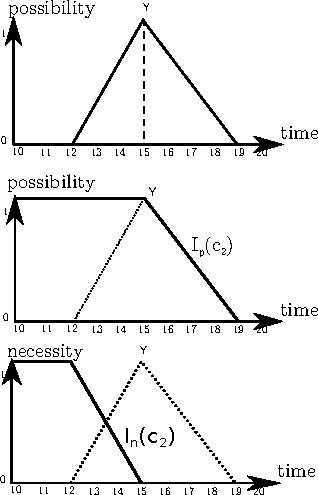
\includegraphics[scale=1]{./graphs/open-time-interval.pdf}
\label{fig:example-open-time-interval}
}
\end{center}
%\centerline{ 
\psfig{file=./graphs/Y-time-point.eps}}
\vspace*{10pt}
\fcaption{Possibility distribution for $Y$, and possibility and necessity measures for the open ill-known point, $X$}
\vspace*{13pt}


\vglue13pt
%\begin{table}[htbp]
\tcap{Relations for the $\Open(C)$ function.}
\centerline{\small Relations}
\vglue-6pt
\centerline{\small\baselineskip=13pt
\begin{tabular}{c c c}\\
\hline
$R$ & $\Rp$ & $\Rn$\\ \hline
$<$ & $>$ & $\leq$ \\
$\leq$ & $\geq$ & $<$ \\
$>$ & $<$ & $\geq$ \\
$\geq$ & $\leq$ & $>$ \\
\hline\\
\end{tabular}
\label{tbl:open-pos-nec-rels}
}



\subsubsection{\label{subsubsec:ill-known-time-interval-datatypes}Datatypes}
In order to represent properly an ill-known time interval in a database, some datatypes are needed. Because of the ill-known constraints, not all the combinations of datatypes for each ill-known time point (see Table \ref{tbl:time-point-types}) are allowed. Table \ref{tbl:time-interval-types} shows all the possible combinations for the datatypes for an ill-known time interval denoted by $\left[X, Y\right]$.

\vglue13pt
%\begin{table}[htbp]
\tcap{Data types for an ill-known time interval $\left[X, Y\right]$.}
\centerline{\small DATA TYPES}
\vglue-6pt
\centerline{\small\baselineskip=13pt
\begin{tabular}{c c p{2cm}}\\
\hline
$X$  & $Y$  & Description\\
\hline
$\lbrace1,2 \rbrace$ & $\lbrace1,2 \rbrace$ &  an ill-known time interval.\\
3 & 3 & An unknown time interval. \\
$\FB$ & $\lbrace1,2 \rbrace$ & a left-open time interval.\\
$\lbrace1,2 \rbrace$ & $\UC$ & a right-open time interval.\\
\hline\\
\end{tabular}
\label{tbl:time-interval-types}
}

\subsection{\label{subsec:fuzzy-allen-relations}Allen's relations}

\vglue13pt
%\begin{table}[htbp]
\tcap{\label{tbl:fuzzy-allen-relations}Constructs of constraints related to their respective Allen relations, as used in the presented work. In this table, the ill-known time interval $J = \left[X, Y\right]$ in a record $r$ has a start point described by possibilistic variable $X$ and an end point described by possibilistic variable $Y$. The crisp time interval in the user's temporal demand is denoted $I$.}
\centerline{\small Relations}
\vglue-6pt
\centerline{\small\baselineskip=13pt
\begin{tabular}{c p{4cm} }\\
\hline
Allen Relation & Construct of constraints\\
\hline
I before J & $C_1 \triangleq \left(<,X\right)$ \\
\hline
I equal J & $\left(C_1 \triangleq \left(\geq,X\right)\right) \wedge \neg \left(C_2 \triangleq \left(\neq,X\right) \right) \wedge \left(C_3 \triangleq \left(\leq,Y\right) \right) \wedge \neg \left(C_4 \triangleq \left(\neq,Y\right)\right)$ \\
\hline
I meets J & $\left(C_1 \triangleq \left(\leq,X\right)\right) \wedge \neg \left(C_2 \triangleq \left(\neq,X\right) \right)$ \\
\hline
I overlaps J & $\left(C_1 \triangleq \left(<,Y\right)\right) \wedge \neg \left(C_2 \triangleq \left(\leq,X\right) \right) \wedge \neg \left(C_3 \triangleq \left(\geq,X\right) \right)$ \\
\hline
I during J & $\left( \left (C_1 \triangleq \left(>,X\right) \right) \wedge \left(C_2 \triangleq \left(\leq,Y\right) \right) \right) \vee \left( \left(C_3 \triangleq \left(\geq,X\right) \right) \wedge  \left(C_4 \triangleq \left(<,Y\right) \right) \right)$ \\
\hline
I starts J & $\left(C_1 \triangleq \left(\geq,X\right) \right) \wedge \neg \left(C_2\triangleq \left(\neq,X\right)\right)$ \\
\hline
I finishes J & $\left(C_1 \triangleq \left(\leq,Y\right) \right) \wedge \neg \left(C_2\triangleq \left(\neq,Y\right)\right)$ \\
\hline\\
\end{tabular}
}

%\subsection{\label{subsec:time-interval-constraint}Ill-known valid time-interval}
%The representation of a possibilistic valid-time interval is given by two ill-known points: $\left[S,E \right]$ the starting and ending points respectively.  
%
%
%A valid temporal interval $\left[S,E\right]$ in the system is a combination for the values of $S$,$E$. Note that the only allowed combination of types is shown in table \ref{tbl:valid-time-interval}. 


\section{\label{sec:temporal-model}Possibilistic Valid-Time Model for Relational DBs}
%%%%%%%%%%%%%%%%%%%%%%%%%%%%%%%%
%
% Temporal model.tex
%
%%%%%%%%%%%%%%%%%%%%%%%%%%%%%%%



%
%\vglue13pt
%%\begin{table}[htbp]
%\tcap{Valid-Time interval data types}
%\centerline{\small VALID TIME DATA TYPES}
%\vglue-6pt
%\centerline{\small\baselineskip=13pt
%\begin{tabular}{c p{2cm} p{2cm}}\\
%\hline
%Type for S & Type for E & Semantics \\
%\hline
%Unknown & Unkown & Unknown interval. \\
%\hline
%1,2 & 1,2 & A possibilistic time interval. \\
%\hline\\
%\end{tabular}
%\label{tbl:valid-time-interval}}
%%\end{table}
%
%The following is a study of the constraints in the range of values for both starting and ending times to represent a valid time interval.
%
%The time period inside a valid time interval is denoted by two constraints:
%\begin{eqnarray}
%C_1\stackrel{\triangle}{=}\left(\geq,X\right)\\
%C_2\stackrel{\triangle}{=}\left(\leq,Y\right).
%\end{eqnarray}
%Applying the inference of uncertainty as proposed in our general reasoning, we find for the first constraint that:
%\begin{eqnarray}
%\Pos\left(C_1([a,b])\right) &=& \min_{r\in[a,b]}\Big(\sup_{r\leq w}\pi_{X}(w)\Big)\\
%\Nec\left(C_1([a,b])\right) &=& \min_{r\in[a,b]}\Big(\inf_{r>w}1-\pi_{X}(w)\Big)
%\end{eqnarray}
%which can be simplified to:
%\begin{eqnarray}
%\Pos\left(C_1([a,b])\right) &=& \sup_{a\leq w}\pi_{X}(w)\\
%\Nec\left(C_1([a,b])\right) &=& \inf_{a>w}1-\pi_{X}(w).
%\end{eqnarray}
%For the second constraint, we find that:
%\begin{eqnarray}
%\Pos\left(C_2([a,b])\right) &=& \min_{r\in[a,b]}\Big(\sup_{r\geq w}\pi_{Y}(w)\Big)\\
%\Nec\left(C_2([a,b])\right) &=& \min_{r\in[a,b]}\Big(\inf_{r<w}1-\pi_{Y}(w)\Big)
%\end{eqnarray}
%which can be simplified to:
%\begin{eqnarray}
%\Pos\left(C_2([a,b])\right) &=& \sup_{b\geq w}\pi_{Y}(w)\\
%\Nec\left(C_2([a,b])\right) &=& \inf_{b<w}1-\pi_{Y}(w).
%\end{eqnarray}
%The uncertainty about the inclusion of an interval $I=[a,b]$ in the interval with ill-known boundaries can now be found by evaluating $[a,b]$ against the evaluation function $\lambda$ with $\bool=\wedge$. Application of \eqref{eq:conjunctive1} and \eqref{eq:conjunctive2} leads to:
%\begin{eqnarray}
%\Pos\left(\lambda([a,b])\right)&=&\min\bigg(\Pos(C_1([a,b])),\Pos(C_2([a,b]))\bigg)\\
%\Nec\left(\lambda([a,b])\right)&=&\min\bigg(\Nec(C_1([a,b])),\Nec(C_2([a,b]))\bigg).
%\end{eqnarray}
%These last expressions can also be expanded as:
%\begin{eqnarray}
%\label{eq:interval-pos}
%\Pos\left(\lambda([a,b])\right)&=&\min\bigg(\sup_{a\leq w}\pi_{X}(w),\sup_{b\geq w}\pi_{Y}(w)\bigg)\\
%\label{eq:interval-nec}
%\Nec\left(\lambda([a,b])\right)&=&\min\bigg(\inf_{a>w}1-\pi_{X}(w),\inf_{b<w}1-\pi_{Y}(w)\bigg).
%\end{eqnarray}
%Note that the interval $[X,Y]$ used here, is certainly not a fuzzy interval. Instead, we are dealing with an ill-known interval, i.e. it is a crisp interval, but it is partially unknown which values are in this interval. The uncertainty stems from the fact that the interval boundaries are ill-known.
%
%Within this framework for the reasoning of the knowledge about the interval, we are going to study the semantics from the point of view of the valid time as well as from the point of view of the temporal database.
%
%\subsubsection{S = Unknown, E = Unknown}
%Consider that the possibility distribution for S is Unknown and for E is also Unknown. The possibility distributions are $\pi_S$ and $\pi_E$ respectively:
%
%\begin{eqnarray}
%\pi_{S}(t \in \T) = 1\\
%\pi_{E}(t \in \T) = 1
%\end{eqnarray}
%
%Therefore the constraints $C_1$ and $C_2$ are:
%
%\begin{eqnarray}
%\Pos\left(C_1([a,b])\right) &=& \sup_{a\leq w}\pi_{S}(w) = 1\\
%\Nec\left(C_1([a,b])\right) &=& \inf_{a>w}1-\pi_{S}(w) = 0\\
%\Pos\left(C_2([a,b])\right) &=& \sup_{b\geq w}\pi_{E}(w)=1\\
%\Nec\left(C_2([a,b])\right) &=& \inf_{b<w}1-\pi_{E}(w)=0
%\end{eqnarray}
%
%
%\begin{eqnarray}
%\Pos\left(\lambda([a,b])\right)&=&\min\bigg(\sup_{a\leq w}\pi_{S}(w),\sup_{b\geq w}\pi_{E}(w)\bigg) \\
%&=& \min(1,1)  = 1\\
%\Nec\left(\lambda([a,b])\right)&=&\min\bigg(\inf_{a>w}1-\pi_{S}(w),\inf_{b<w}1-\pi_{E}(w)\bigg)\\
%&=& \min(0,0) = 0
%\end{eqnarray}
%
%\begin{example}
%A constant object in the database. It is an object that is always valid in the database.
%The main issue in a valid time database is that the update sentence have to modify the starting or ending point distribution. The most natural way to convert a snapshot database to a temporal database is to consider the objects belonging to the interval [Unknown, Unknown].
%\end{example}
%
%\subsubsection{[Unknown,value] or [value,Unknown]}
%These two cases are managed in this section. Here we will note $\pi_{S}(t)$ or $\pi_{E}(t)$ as the possibility distribution for 'value' in the starting or ending points.
%
%First of all the case [Unknown,value] in \eqref{eq:interval-pos} and in \eqref{eq:interval-nec}:
%
%\begin{eqnarray}
%\Pos\left(\lambda([a,b])\right)&=&\min (1,\sup_{b\geq w}\pi_{E}(w))\\
% &=& \sup_{b\geq w}\pi_{E}(w)\\
%\Nec\left(\lambda([a,b])\right)&=&\min (0,\inf_{b<w}1-\pi_{E}(w))\\
%&=& 0
%\end{eqnarray}
%
%Similarily for [value,Unknown] the possibility and neccesity are:
%\begin{eqnarray}
%\Pos\left(\lambda([a,b])\right)&=&\min (\sup_{a\leq w}\pi_{S}(w),1)\\
% &=& \sup_{a\leq w}\pi_{S}(w)\\
%\Nec\left(\lambda([a,b])\right)&=&\min (\inf_{a>w}1-\pi_{S}(w),0)\\
%&=& 0
%\end{eqnarray}
%
%The semantics for an object with valid time given by [Unknown,value] is an object that has been valid from the beggining to an ending time. Analogously, the semantics for an object with a valid time given by the interval [value,Unknown] is an object that it is still valid in the database. 
%
%
%\subsubsection{[Undefined,Undefined]}
%Maybe this combination has no sense for a valid time object. The possibility distributions for both starting and ending points are:
%
%\begin{eqnarray}
%\pi_{S}(t \in \T) = 0\\
%\pi_{E}(t \in \T) = 0
%\end{eqnarray}
%
%Therefore the constraints $C_1$ and $C_2$ are:
%
%\begin{eqnarray}
%\Pos\left(C_1([a,b])\right) &=& \sup_{a\leq w}\pi_{S}(w) = 0\\
%\Nec\left(C_1([a,b])\right) &=& \inf_{a>w}1-\pi_{S}(w) = 1\\
%\Pos\left(C_2([a,b])\right) &=& \sup_{b\geq w}\pi_{E}(w)=0\\
%\Nec\left(C_2([a,b])\right) &=& \inf_{b<w}1-\pi_{E}(w)=1
%\end{eqnarray}
%
%Taking these values into  \eqref{eq:interval-pos} and in \eqref{eq:interval-nec}:
%\begin{eqnarray}
%\Pos\left(\lambda([a,b])\right)&=&\min (0,0)\\
% &=& 0\\
%\Nec\left(\lambda([a,b])\right)&=&\min (1,1)\\
%&=& 1
%\end{eqnarray}
%
%\textcolor{red}{TAKE A LOOK INTO THIS}
%
%Which is an inconsistency.
%
%\subsection{[Undefined,value] or [value,Undefined]}
%
%The possibility and neccesity measures for [Undefined,value] are :
%\begin{eqnarray}
%\Pos\left(\lambda([a,b])\right)&=&\min (0,\sup_{b\geq w}\pi_{E}(w))\\
% &=& 0\\
%\Nec\left(\lambda([a,b])\right)&=&\min (1,\inf_{b<w}1-\pi_{E}(w))\\
%&=& \inf_{b<w}1-\pi_{E}(w)
%\end{eqnarray}
%
%The other way around, [value,Undefined]:
%\begin{eqnarray}
%\Pos\left(\lambda([a,b])\right)&=&\min (\sup_{a\leq w}\pi_{S}(w),0)\\
% &=& 0\\
%\Nec\left(\lambda([a,b])\right)&=&\min (\inf_{a>w}1-\pi_{S}(w),1)\\
%&=& \inf_{a>w}1-\pi_{S}(w)
%\end{eqnarray}
%
%\textcolor{red}{TAKE A LOOK INTO THIS}
%This is also an inconsistency.
%
%\subsubsection{[NULL,NULL] and maybe any combination with NULL}
%I think the framework we have can not deal with NULL computations. Maybe just for non-specified time or something like that.
%
%\subsubsection{[Undefined,Unknown] or [Unknown,Undefined]}
%The semantic for this could be also unconsistent.
%
%
%\begin{example}
%Consider a snapshot database (table \ref{tbl:snapshot-car-models}) that stores information about car models. The primary key is given by the set $\lbrace$ Brand, Model $\rbrace$.
%
%\vglue13pt
%%\begin{table}[htbp]
%\tcap{Car model snapshot database}
%\centerline{\small CAR MODELS}
%\vglue-6pt
%\centerline{\small\baselineskip=13pt
%\begin{tabular}{c c c}\\
%\hline
%\textbf{Brand} & \textbf{Model} & Segment \\
%\hline
%Peugeot & 205 & B \\
%Peugeot & 206 & B \\
%Peugeot & 207 & B \\
%Peugeto & 208 & B \\
%Citroen & C2 & B \\
%\hline\\
%\end{tabular}
%\label{tbl:snapshot-car-models}
%}
%
%Consider now that the user wants to make that table a valid-time table, then, from the point of view of the storage, the following changes should be done:
%
%\begin{itemize}
%\item
%A new definition for the primary key, including a version field.
%\item
%The addition of two new columns to store the valid-time interval. By default the initial values are Unknown for both starting and ending points of the interval.
%\end{itemize}
%Therefore, the table \ref{tbl:snapshot-car-models} is transformed into table \ref{tbl:initial-valid-time-car-models}:
%
% \vglue13pt
%%\begin{table}[htbp]
%\tcap{Car model valid-time database. Note that U is the abbreviation for the Unknown constant.}
%\centerline{\small VALID TIME CAR MODELS}
%\vglue-6pt
%\centerline{\small\baselineskip=13pt
%\begin{tabular}{c c c c c c}\\
%\hline
%\textbf{Brand} & \textbf{Model} & \textbf{VersionID} & Segment & S & E \\
%\hline
%Peugeot & 205 & 001 & B & U & U \\
%Peugeot & 206 & 001 & B & U & U \\
%Peugeot & 207 & 001 & B & U & U \\
%Peugeto & 208 & 001 & B & U & U \\
%Citroen & C2 & 001 & B & U & U \\
%\hline\\
%\end{tabular}
%\label{tbl:initial-valid-time-car-models}
%}
%
%
%
%\end{example}


\subsection{\label{subsec:temporal-model}The generalized temporal model}

\begin{definition}
Generalized fuzzy temporal domain.\\
If $\T$ is the temporal domain, $\tilde \Pow\left( \T\right)$ is the set of all possibility distributions defined on $\T$.
The \textbf{Generalized Fuzzy Temporal Domain}, $\T_G$ is
\begin{equation}
\T_G \subseteq \left \lbrace \tilde \Pow\left( \T\right) \cup NULL \right \rbrace
\end{equation}
\end{definition}

%\section{\label{sec:querying}Querying}
%\input{./sources/querying.tex}

\section{\label{sec:conclusions}Conclusions}
In this paper, a comparison is presented between two different frameworks designed to represent time intervals subject to uncertainty and evaluate temporal relationships between such intervals and crisp intervals: the triangular model (TM) framework and the ill-known constraint (IKC) framework. It is concluded that:

\begin{itemize}
	\item With respect to representation, both frameworks differ only slightly, with the TM framework allowing easier human assessments, due to its approach including visualization.
	\item With respect to temporal relationship evaluation, the TM framework allows easy human assessments in several situations, but the IKC framework seems more fitted for complex reasoning, due to its modular build.
\end{itemize}

Future research will deal with the evaluation of temporal relationships between several time intervals subject to uncertainty and with querying aspects in both frameworks.

%\subsection{Sub-headings}
%%\vspace*{-4pt}  %only when needed
%Sub-headings should be typeset in bolditalic with the first
%letter of first word capitalized and section number in boldface.
%
%%\vspace*{-1pt}  %only when needed
%\subsubsection{Sub-subheadings}
%%\vspace*{-4pt}  %only when needed
%
%Typeset in italic (Section No. to be in Roman) and capitalize
%the first letter of the first word only.
%
%%\vspace*{-1pt}  %only when needed
%\subsection{Numbering and spacing}
%%\vspace*{-4pt}  %only when needed
%
%Sections, sub-sections and sub-subsections are numbered in Arabic.
%Use double spacing after major and subheadings, and single spacing
%after\break sub-subheadings.
%
%%\vspace*{-1pt}  %only when needed
%\subsection{Lists of items}
%%\vspace*{-4pt}  %only when needed
%
%{Lists may be laid out with each item marked by\hfilneg}
%
%\noindent a dot:
%\begin{itemize}
%\item item one,
%\item item two.
%\end{itemize}
%
%\setcounter{footnote}{0}
%\renewcommand{\thefootnote}{\alph{footnote}}
%
%Items may also be numbered in lowercase Roman numerals:
%\begin{enumerate}[(i)]\Nospacing
%\item item one
%\item item two
%    \begin{enumerate}[(a)]\Nospacing
%    \item Lists within lists can be numbered with lowercase Roman letters,
%    \item second item.
%    \end{enumerate}
%\end{enumerate}
%
%\subsection{Running Heads}
%
%Please provide a shortened running head (not more than four words,
%each starting with a Capital) for the title of your paper. This will
%appear with page numbers on the top right-hand side of your paper on
%odd pages.
%
%For the running heads for the authors names should appear on your paper
%on the even  pages. Please apply the following rules for theses running
%heads:
%\begin{itemize}
%\item for one author: only the initial plus the full last name (e.g., D. Ruan),
%\item for two authors: D. Ruan, T. Li,
%\item for three authors or more: D. Ruan \emph{et al.}
%\end{itemize}
%
%\section{Equations}
%
%Displayed equations should be numbered consecutively in each
%section, with the number set flush right and enclosed in
%parentheses.
%\begin{equation}
%\mu(n,t) = \dfrac{\sum^\infty_{i=1} 1(d_i < t, N(d_i) = n)}
%{\int^t_{\sigma=0} 1(N(\sigma) = n)\mathrm{d}\sigma}\,\, .
%\label{this}
%\end{equation}
%Equations should be referred to in abbreviated form,
%e.g.~``Eq.~(\ref{this})'' or ``(2)''. In multiple-line equations,
%the number should be given on the last line.
%
%Displayed equations are to be centered on the page width.
%Standard English letters like x are to appear as $x$ (italicized)
%in the text if they are used as mathematical symbols. Punctuation
%marks are used at the end of equations as if they appeared directly in the text.
%
%\begin{theorem}
%Theorems, lemmas, etc. are to be numbered consecutively in the
%paper, just by using \\
%\verb+\begin{env}My text here...\end{env}+\\
%for the environments \emph{theorem}, \emph{lemma},
%\emph{proposition}, and \emph{corollary}.\\
%\end{theorem}
%
%\vspace*{-5pt}
%
%\begin{proof}
%Proofs are produced with the command\\
%\verb+\begin{proof}{My proof...}\end{proof}+.\\
%It should end with\ $\qed$\kern0.3pt.
%\end{proof}
%
%\section{Illustrations and Photographs}
%
%Figures are to be inserted in the text nearest their first reference.
%Original india ink drawings or glossy prints are preferred. Please
%send one set of originals with copies. If the author requires the
%publisher to reduce the figures, ensure that {the figures (including
%letterings and numbers) are large enough to be\hfilneg}
%
%%\begin{figure}[htbp] %ORIGINAL SIZE: width=1.4TRUEIN; height=1.5TRUEIN
%%\vspace*{13pt}
%%\centerline{\psfig{file=ap-ijcis.eps}} %100 percent
%\vspace*{10pt}
%\fcaption{Labeled tree {\it T}.}
%%\end{figure}
%\vspace*{13pt}
%
%\noindent
%clearly seen after reduction. If photographs are to be used, only
%black and white ones are acceptable.
%
%Figures are to be sequentially numbered in Arabic numerals. The
%caption must be placed below the figure. For those figures with
%multiple parts which appear on different pages, it is best to
%place the full caption below the first part, and have
%e.g.~``Fig.~1. ({\it Continued})'' below the last part. Typeset
%in 9~pt Times Roman with baselineskip of 11~pt. Use double
%spacing between a caption and the text that follows immediately.
%
%Previously published material must be accompanied by written
%permission from the author and publisher.
%
%\section{Tables}
%
%Tables should be inserted in the text as close to the point of
%reference as possible. Some space should be left above and below
%the table. Tables should be numbered sequentially in the text in
%Arabic numerals. Captions are to be centralized above the
%tables. Typeset tables and captions in 9~pt Times Roman with
%baselineskip of 11~pt.
%
%If tables need to extend over to a second page, the continuation
%of the table should be preceded by a caption, e.g.~``Table~2.
%({\it Continued})''
%
%\vglue13pt
%%\begin{table}[htbp]
%\tcap{Number of tests for WFF triple NA = 5, or\break NA = 8.}
%\centerline{\small NP}
%\vglue-6pt
%\centerline{\small\baselineskip=13pt
%\begin{tabular}{l c c c c c}\\
%\hline
%{} &{} &3 &4 &8 &10\\
%\hline
%{} &\phantom03 &1200 &2000 &\phantom02500 &\phantom03000\\
%NC &\phantom05 &2000 &2200 &\phantom02700 &\phantom03400\\
%{} &\phantom08 &2500 &2700 &16000 &22000\\
%{} &10 &3000 &3400 &22000 &28000\\
%\hline\\
%\end{tabular}}
%%\end{table}
%
%\section{References}
%
%References in the text are to be numbered consecutively in Arabic
%numerals, in the order of first appearance. They are to be cited as
%superscripts without parentheses or brackets after punctuation marks
%like commas and periods but before punctuation marks like colons,
%semi-colons and question marks. Where superscripts might cause
%ambiguity, cite references in parentheses in abbreviated form,
%e.g.~(Ref.~12).
%
%\section{Footnotes}
%
%Footnotes should be numbered sequentially in superscript
%lowercase Roman letters.\fnm{a}\fnt{a}{Footnotes should be
%typeset in 8~pt Times Roman at the bottom of the page.}
%
%\section*{Note Added}
%
%Additional note can be added before Acknowledgment.
%
%\section*{Acknowledgments}
%
%This section should come before the References. Funding
%information may also be included here.
%
%\appendix{}
%
%Appendices should be used only when absolutely necessary. They should
%come immediately\break before the References. If there is more than
%one appendix, number them alphabetically. Number%\break
%displayed equations occurring in the Appendix in this way, e.g.~(\ref{that}),
%(A.2), etc.
%\begin{equation}
%\mu(n,t) = {\displaystyle\sum^\infty_{i=1} 1(d_i < t, N(d_i) = n) \over
%\displaystyle\int^t_{\sigma=0} 1(N(\sigma) = n)d\sigma}\,\, .\label{that}
%\end{equation}
%
%\section*{References}
%References are to be listed in the order cited in the text. Use the style shown
%in the following examples. For journal names, use the standard abbreviations.
%Typeset references in 9~pt Times Roman.
%
%%----------------------------- END BODY OF TEXT -----------------------------
%
%\begin{thebibliography}{000}
%\bibitem{1}
%J. J. Hopfield, ``Neurons with graded response have collective
%computational properties like two-state neurons,'' {\it Proc. Natl. Acad. Sci.},
%{\bf 81}, 3088--3092 (1984).
%
%\bibitem{2}
%D. W. Tank and J. J. Hopfield, ``Simple `neural' optimization networks:
%An A/D converter, signal decision circuit, and a linear programming circuit,''
%{\it IEEE Trans. on Circuits and Systems}, {\bf 33}, 533--541 (1986).
%
%\bibitem{3}
%Y. S. Foo and Y. Takefuji, ``Integer linear programming neural networks for
%job-shop scheduling,'' {\it Proc. IEEE Intl. Conf. on Neural Networks},
%{\bf II}, 341--348 (1988).
%%\phantom{00}
%\label{\labart-LastPage}
%\end{thebibliography}

\section*{Acknowledgments}
Part of the researchers are supported by the grant BES-2009-013805 in the project TIN2008-02066: \emph{Fuzzy Temporal Information Treatment in RDBMS} and  the project P07-TIC-03175: \emph{Representaci\'on y Manipulaci\'on de Objetos Imperfectos en Problemas de Integraci\'on de Datos: Una Aplicaci\'on a los Almacenes de Objetos de Aprendizaje}.





\section*{References}
\bibliographystyle{spmpsci}
\bibliography{biblio}

\end{multicols}
\end{document}
